\documentclass[]{article}
\usepackage{lmodern}
\usepackage{amssymb,amsmath}
\usepackage{ifxetex,ifluatex}
\usepackage{fixltx2e} % provides \textsubscript
\ifnum 0\ifxetex 1\fi\ifluatex 1\fi=0 % if pdftex
  \usepackage[T1]{fontenc}
  \usepackage[utf8]{inputenc}
\else % if luatex or xelatex
  \ifxetex
    \usepackage{mathspec}
  \else
    \usepackage{fontspec}
  \fi
  \defaultfontfeatures{Ligatures=TeX,Scale=MatchLowercase}
\fi
% use upquote if available, for straight quotes in verbatim environments
\IfFileExists{upquote.sty}{\usepackage{upquote}}{}
% use microtype if available
\IfFileExists{microtype.sty}{%
\usepackage{microtype}
\UseMicrotypeSet[protrusion]{basicmath} % disable protrusion for tt fonts
}{}
\usepackage[margin=1in]{geometry}
\usepackage{hyperref}
\hypersetup{unicode=true,
            pdftitle={Managing for ecological surprises in metapopulations},
            pdfborder={0 0 0},
            breaklinks=true}
\urlstyle{same}  % don't use monospace font for urls
\usepackage{color}
\usepackage{fancyvrb}
\newcommand{\VerbBar}{|}
\newcommand{\VERB}{\Verb[commandchars=\\\{\}]}
\DefineVerbatimEnvironment{Highlighting}{Verbatim}{commandchars=\\\{\}}
% Add ',fontsize=\small' for more characters per line
\usepackage{framed}
\definecolor{shadecolor}{RGB}{248,248,248}
\newenvironment{Shaded}{\begin{snugshade}}{\end{snugshade}}
\newcommand{\AlertTok}[1]{\textcolor[rgb]{0.94,0.16,0.16}{#1}}
\newcommand{\AnnotationTok}[1]{\textcolor[rgb]{0.56,0.35,0.01}{\textbf{\textit{#1}}}}
\newcommand{\AttributeTok}[1]{\textcolor[rgb]{0.77,0.63,0.00}{#1}}
\newcommand{\BaseNTok}[1]{\textcolor[rgb]{0.00,0.00,0.81}{#1}}
\newcommand{\BuiltInTok}[1]{#1}
\newcommand{\CharTok}[1]{\textcolor[rgb]{0.31,0.60,0.02}{#1}}
\newcommand{\CommentTok}[1]{\textcolor[rgb]{0.56,0.35,0.01}{\textit{#1}}}
\newcommand{\CommentVarTok}[1]{\textcolor[rgb]{0.56,0.35,0.01}{\textbf{\textit{#1}}}}
\newcommand{\ConstantTok}[1]{\textcolor[rgb]{0.00,0.00,0.00}{#1}}
\newcommand{\ControlFlowTok}[1]{\textcolor[rgb]{0.13,0.29,0.53}{\textbf{#1}}}
\newcommand{\DataTypeTok}[1]{\textcolor[rgb]{0.13,0.29,0.53}{#1}}
\newcommand{\DecValTok}[1]{\textcolor[rgb]{0.00,0.00,0.81}{#1}}
\newcommand{\DocumentationTok}[1]{\textcolor[rgb]{0.56,0.35,0.01}{\textbf{\textit{#1}}}}
\newcommand{\ErrorTok}[1]{\textcolor[rgb]{0.64,0.00,0.00}{\textbf{#1}}}
\newcommand{\ExtensionTok}[1]{#1}
\newcommand{\FloatTok}[1]{\textcolor[rgb]{0.00,0.00,0.81}{#1}}
\newcommand{\FunctionTok}[1]{\textcolor[rgb]{0.00,0.00,0.00}{#1}}
\newcommand{\ImportTok}[1]{#1}
\newcommand{\InformationTok}[1]{\textcolor[rgb]{0.56,0.35,0.01}{\textbf{\textit{#1}}}}
\newcommand{\KeywordTok}[1]{\textcolor[rgb]{0.13,0.29,0.53}{\textbf{#1}}}
\newcommand{\NormalTok}[1]{#1}
\newcommand{\OperatorTok}[1]{\textcolor[rgb]{0.81,0.36,0.00}{\textbf{#1}}}
\newcommand{\OtherTok}[1]{\textcolor[rgb]{0.56,0.35,0.01}{#1}}
\newcommand{\PreprocessorTok}[1]{\textcolor[rgb]{0.56,0.35,0.01}{\textit{#1}}}
\newcommand{\RegionMarkerTok}[1]{#1}
\newcommand{\SpecialCharTok}[1]{\textcolor[rgb]{0.00,0.00,0.00}{#1}}
\newcommand{\SpecialStringTok}[1]{\textcolor[rgb]{0.31,0.60,0.02}{#1}}
\newcommand{\StringTok}[1]{\textcolor[rgb]{0.31,0.60,0.02}{#1}}
\newcommand{\VariableTok}[1]{\textcolor[rgb]{0.00,0.00,0.00}{#1}}
\newcommand{\VerbatimStringTok}[1]{\textcolor[rgb]{0.31,0.60,0.02}{#1}}
\newcommand{\WarningTok}[1]{\textcolor[rgb]{0.56,0.35,0.01}{\textbf{\textit{#1}}}}
\usepackage{graphicx,grffile}
\makeatletter
\def\maxwidth{\ifdim\Gin@nat@width>\linewidth\linewidth\else\Gin@nat@width\fi}
\def\maxheight{\ifdim\Gin@nat@height>\textheight\textheight\else\Gin@nat@height\fi}
\makeatother
% Scale images if necessary, so that they will not overflow the page
% margins by default, and it is still possible to overwrite the defaults
% using explicit options in \includegraphics[width, height, ...]{}
\setkeys{Gin}{width=\maxwidth,height=\maxheight,keepaspectratio}
\IfFileExists{parskip.sty}{%
\usepackage{parskip}
}{% else
\setlength{\parindent}{0pt}
\setlength{\parskip}{6pt plus 2pt minus 1pt}
}
\setlength{\emergencystretch}{3em}  % prevent overfull lines
\providecommand{\tightlist}{%
  \setlength{\itemsep}{0pt}\setlength{\parskip}{0pt}}
\setcounter{secnumdepth}{0}
% Redefines (sub)paragraphs to behave more like sections
\ifx\paragraph\undefined\else
\let\oldparagraph\paragraph
\renewcommand{\paragraph}[1]{\oldparagraph{#1}\mbox{}}
\fi
\ifx\subparagraph\undefined\else
\let\oldsubparagraph\subparagraph
\renewcommand{\subparagraph}[1]{\oldsubparagraph{#1}\mbox{}}
\fi

%%% Use protect on footnotes to avoid problems with footnotes in titles
\let\rmarkdownfootnote\footnote%
\def\footnote{\protect\rmarkdownfootnote}

%%% Change title format to be more compact
\usepackage{titling}

% Create subtitle command for use in maketitle
\providecommand{\subtitle}[1]{
  \posttitle{
    \begin{center}\large#1\end{center}
    }
}

\setlength{\droptitle}{-2em}

  \title{Managing for ecological surprises in metapopulations}
    \pretitle{\vspace{\droptitle}\centering\huge}
  \posttitle{\par}
  \subtitle{Supplemental materials: Model details \& results}
  \author{\textup{Kyle L. Wilson$^a$}\footnote{Corresponding author - email:
  \href{mailto:kl_wilson@sfu.ca}{\nolinkurl{kl\_wilson@sfu.ca}}}\textup{, Alex Sawyer$^a$, Anna Potapova$^a$, Colin J. Bailey$^a$, Elissa Sweeney-Bergen$^a$, Emma E. Hodgson$^a$, Kara J. Pitman$^a$, Karl Seitz$^a$, Lauren Law$^a$, Luke Warkentin$^a$, Samantha M. Wilson$^a$, William I. Atlas$^a$, Daniella LoScerbo$^b$, Douglas C. Braun$^c$, Matthew R. Sloat$^d$, M. Tim Tinker$^e$, and Jonathan W. Moore$^{a,b}$}\\
~\\
\textup{$^a$Earth to Ocean Research Group, Simon Fraser University}\\
\textup{$^b$Resource and Environmental Management, Simon Fraser University}\\
\textup{$^c$Fisheries and Oceans Canada}\\
\textup{$^d$Wild Salmon Center}\\
\textup{$^e$Ecology and Evolutionary Biology, University of California Santa Cruz}}
    \preauthor{\centering\large\emph}
  \postauthor{\par}
      \predate{\centering\large\emph}
  \postdate{\par}
    \date{22 July 2019}

\usepackage{wrapfig}
\usepackage{lipsum}
\usepackage{float}
\usepackage{lineno}
\usepackage{amsmath}
\linenumbers
\renewcommand{\thefigure}{S\arabic{figure}}
\renewcommand{\thetable}{S\arabic{table}}
\usepackage{fancyhdr}

\begin{document}
\maketitle

\centering
\raggedright
\tableofcontents
\newpage

\pagestyle{fancy}
\fancyhead[LO,LE]{Wilson \textit{et al.}}
\fancyhead[RO,RE]{\textbf{Appendix A}: Managing ecological surprises}

\hypertarget{metapopulation-model}{%
\subsection{Metapopulation model}\label{metapopulation-model}}

\hypertarget{local-metapopulation-dynamics}{%
\subsubsection{Local \& metapopulation
dynamics}\label{local-metapopulation-dynamics}}

Our metapopulation is defined by a set of local populations \(N_p\) for
a species with a one year generation time with time-dynamics that
follows birth (i.e., recruitment \emph{R}), immigration, death, and
emigration (BIDE) processes typical to metapopulation theory (Hanski
1998):

\begin{align}
N_{i{t+1}}= R_{it}\epsilon_{it}+I_{it}-D_{it}-E_{it}
\end{align}

where \(N_{it+1}\) is the number of adults in patch \emph{i} at time
\emph{t}, \(R_{it}\) is number of recruits, \(I_{it}\) is number of
recruits immigrating into patch \emph{i} from any other patch,
\(D_{it}\) is number of recruits that die due to disturbance regime,
\(E_{it}\) is the number of recruits emigrating from patch \emph{i} into
any other patch, and \(\epsilon_{it}\) is stochasticity in recruitment.

Resoure monitoring often occurs at the scale of the metapopulation
(Anderson \emph{et al.} 2015), hence we define metapopulation adults as:

\begin{align}
{MN}_t = \sum_{i=1}^{N_p} N_{it}
\end{align}

with metapopulation recruits:

\begin{align}
MR_t = \sum_{i=1}^{N_p} R_{it}
\end{align}

Local patch recruitment at time \emph{t} depended on adult densities at
\emph{t-1} and followed a reparameterized Beverton-Holt function:

\begin{align}
R_{it}=\cfrac{\alpha_iN_{it-1}}{1+\cfrac{\alpha_i-1}{\beta_i}N_{it-1}}
\end{align}

where \(\alpha_i\) is the recruitment compensation ratio and \(\beta_i\)
is local patch carrying capacity.

Management often monitors metapopulation resources as the aggregate of
all local populations. For example, take a two patch metapopulation
model that varies \(\alpha_i\) and \(\beta_i\) parameters where:

\begin{Shaded}
\begin{Highlighting}[]
\NormalTok{alpha <-}\StringTok{ }\KeywordTok{c}\NormalTok{(}\DecValTok{2}\NormalTok{, }\DecValTok{4}\NormalTok{)}
\NormalTok{beta <-}\StringTok{ }\KeywordTok{c}\NormalTok{(}\DecValTok{100}\NormalTok{, }\DecValTok{200}\NormalTok{)}
\end{Highlighting}
\end{Shaded}

Here, recruitment compensation from local patches \(\alpha_i\) gets
averaged across the metapopulation leading to an average compensation
ratio \(\bar{\alpha}\) of 3. Likewise, the total carrying capacity of
the metapopulation \(\bar{\beta}\) becomes the summation of local patch
carrying capacities \(\sum\beta_i\), which is 300. This scale of
monitoring generates the following local patch and metapopulation
dynamics:

\begin{figure}[H]

{\centering 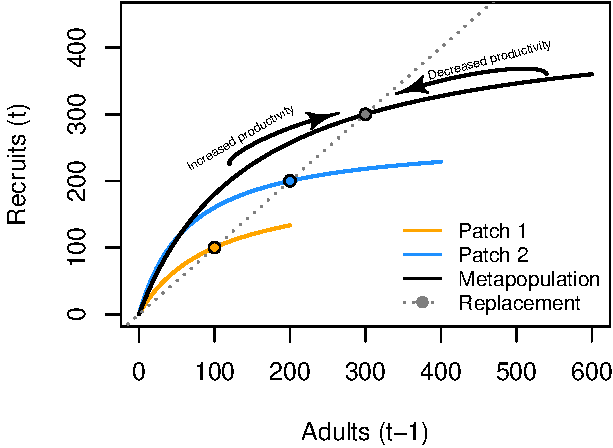
\includegraphics{Managing_for_ecological_surprises_in_metapopulations_files/figure-latex/recruit curves-1} 

}

\caption{Metapopulation and local patch recruitment dynamics.}\label{fig:recruit curves}
\end{figure}

\hypertarget{creating-the-spatial-networks}{%
\subsubsection{Creating the spatial
networks}\label{creating-the-spatial-networks}}

The next aspect to our metapopulation model is connecting the set of
patches to one another (Yeakel \emph{et al.} 2014). We need to specify
the number of patches, their arrangements (i.e., connections), and how
far apart they are from one another. We followed some classic
metapopulation and source-sink arrangements to create four networks that
generalize across a few real-world topologies: a linear habitat network
(e.g., coastline), a dendritic or branching network (e.g., coastal
rivers), a star network (e.g., mountain \& valley, or lake with inlet
tributaries), and a complex network (e.g., terrestrial plants).

To make networks comparable, each spatial network type needs the same
leading parameters (e.g., number of patches \(N_p\) and mean distance
between neighboring patches \(\bar{d}\)). In this case, we set \(N_p\)
to \texttt{16} and \(\bar{d}\) to \texttt{1} unit (distance units are
arbitrary). We used the \texttt{igraph} package (Csardi \& Nepusz 2006)
and some custom code to arrange our spatial networks as the following:

\begin{figure}[H]

{\centering 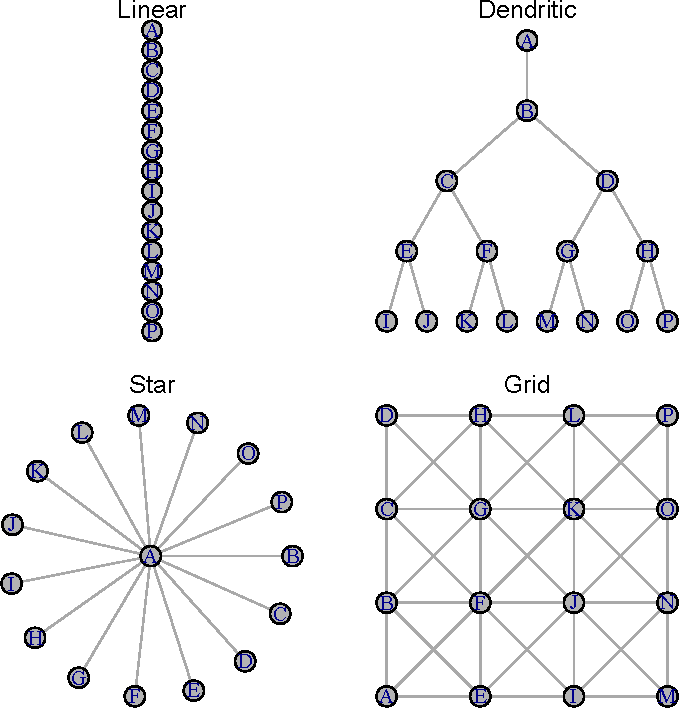
\includegraphics{Managing_for_ecological_surprises_in_metapopulations_files/figure-latex/networks-1} 

}

\caption{Four spatial network topologies.}\label{fig:networks}
\end{figure}

Note that distances between neighbor patches in the above networks are
equal.

\newpage

An example dispersal matrix for the complex network:

\begin{verbatim}
##   A B E F C G D H I J K L M N O P
## A 0 1 1 1 2 2 3 3 2 2 2 3 3 3 3 3
## B 1 0 1 1 1 1 2 2 2 2 2 2 3 3 3 3
## E 1 1 0 1 2 2 3 3 1 1 2 3 2 2 2 3
## F 1 1 1 0 1 1 2 2 1 1 1 2 2 2 2 2
## C 2 1 2 1 0 1 1 1 2 2 2 2 3 3 3 3
## G 2 1 2 1 1 0 1 1 2 1 1 1 2 2 2 2
## D 3 2 3 2 1 1 0 1 3 2 2 2 3 3 3 3
## H 3 2 3 2 1 1 1 0 3 2 1 1 3 2 2 2
## I 2 2 1 1 2 2 3 3 0 1 2 3 1 1 2 3
## J 2 2 1 1 2 1 2 2 1 0 1 2 1 1 1 2
## K 2 2 2 1 2 1 2 1 2 1 0 1 2 1 1 1
## L 3 2 3 2 2 1 2 1 3 2 1 0 3 2 1 1
## M 3 3 2 2 3 2 3 3 1 1 2 3 0 1 2 3
## N 3 3 2 2 3 2 3 2 1 1 1 2 1 0 1 2
## O 3 3 2 2 3 2 3 2 2 1 1 1 2 1 0 1
## P 3 3 3 2 3 2 3 2 3 2 1 1 3 2 1 0
\end{verbatim}

\hypertarget{dispersal}{%
\subsubsection{Dispersal}\label{dispersal}}

Dispersal from patch \emph{i} into patch \emph{j} depends on constant
dispersal rate \(\omega\) (defined as the proportion of total local
recruits that will disperse) and an exponential distance-decay function
between \emph{i} and \emph{j} with distance cost to dispersal \(m\)
following Anderson \emph{et al.} (2015):

\begin{align}
E_{ij(t)}=\omega R_{it}p_{ij}
\end{align}

where \(E_{ij}\) is the total dispersing animals from patch \emph{i}
into patch \emph{j} resulting from dispersal rate \(\omega\), total
number of local recruits \(R_{it}\), and probability of dispersal
between patches \(p_{ij}\):

\begin{align}
p_{ij}=\dfrac{e^{-md_{ij}}}{\sum\limits_{\substack{j=1 \\ j\neq i}}^{N_p} e^{-md_{ij}}}
\end{align}

where \(d_{ij}\) is the pairwise distance between patches, \(m\) is the
distance cost to dispersal. The summation term in the denominator
normalizes the probability of moving to any patch to between 0 and 1
with the constraint that dispersers cannot move back into their home
patch (i.e., \(j\neq i\). With \(\bar{d}= 1\), \(m=0.5\),
\(\omega=0.1\), \(R_{it}=100\) in a linear network:

\begin{figure}[H]

{\centering 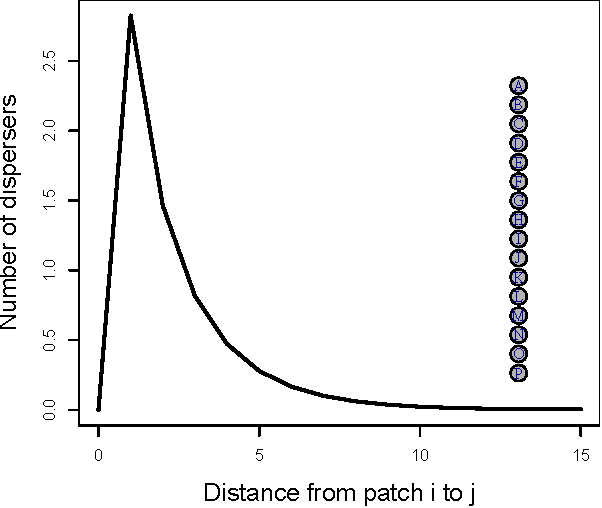
\includegraphics{Managing_for_ecological_surprises_in_metapopulations_files/figure-latex/dispersal-1} 

}

\caption{Example dispersal patterns across linear network.}\label{fig:dispersal}
\end{figure}

\hypertarget{disturbance-regimes}{%
\subsubsection{Disturbance regimes}\label{disturbance-regimes}}

In all scenarios, disturbance was applied after \texttt{50} years of
equilibrating the metapopulaton at pristine conditions. At year
\texttt{51}, we applied the disturbance regime (the regime varied from
\emph{uniform}, \emph{localized, random}, and \emph{localized,
extirpation} - see \emph{Scenarios} below). Disturbance immediately
removes a set proportion of the metapopulation adults at that time
(i.e., \texttt{0.9} of \(MN_{t=51}\)). Once applied, the metapopulation
was no longer disturbed and spatio-temporal recovery dynamics emerged
naturally from these new conditions.

\begin{figure}[H]

{\centering 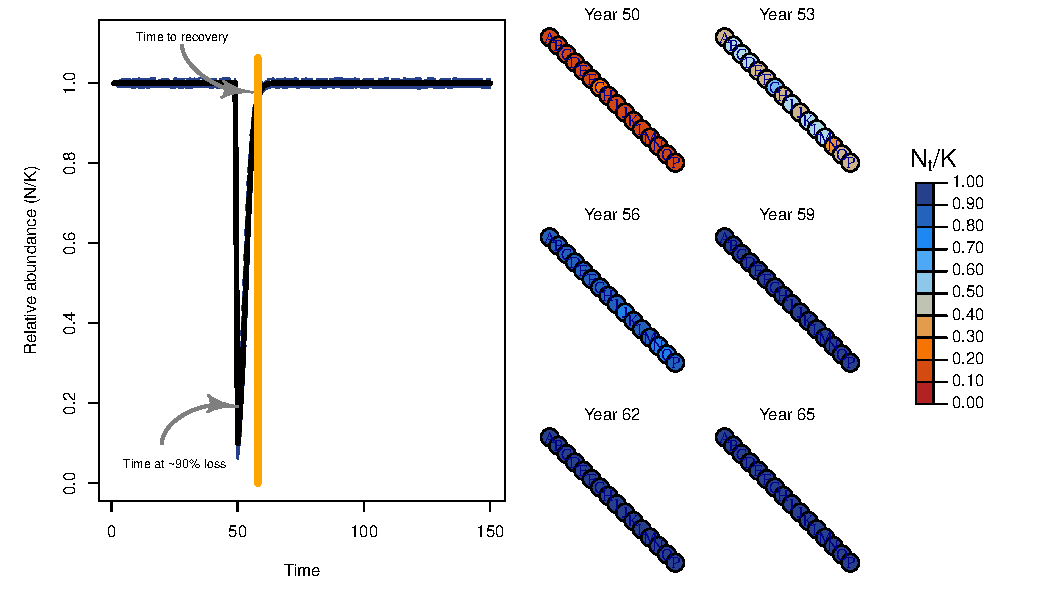
\includegraphics{Managing_for_ecological_surprises_in_metapopulations_files/figure-latex/example disturbance regime-1} 

}

\caption{Recovery regime of metapopulation with linear topology through time (left) and space (right).}\label{fig:example disturbance regime}
\end{figure}

\hypertarget{recruitment-stochasticity}{%
\subsubsection{Recruitment
stochasticity}\label{recruitment-stochasticity}}

Our model allowed for stochastic recruitment that followed a lognormal
distribution with average variation in recruitment of \(\sigma_R\). In
cases of stochastic recruitment, the expected recruitment:

\begin{align}
R_{it}=\cfrac{\alpha_iN_{it-1}}{1+\cfrac{\alpha_i-1}{\beta_i}N_{it-1}}
\end{align}

becomes:

\begin{align}
R_{it}=\cfrac{\alpha_iN_{it-1}}{1+\cfrac{\alpha_i-1}{\beta_i}N_{it-1}}e^{(\epsilon_{it}-\cfrac{ln(\sigma_{R}^2+1)}{2})}
\end{align}

where lognormal deviates for each patch \emph{i} at time \emph{t} are
drawn from a multivariate normal distribution (\emph{MVN}) If
\(\sigma_R\) is low, then metapopulation dynamics approach the
deterministic case. In some scenarios, we evaluate the role of spatially
and/or temporally correlated deviates across the metapopulations to
model potential common drivers affecting metapopulation dynamics (e.g.,
Moran effects). Expected recruitment deviates followed a first-order
autoregression model such that:

\begin{align}
\epsilon_{it}=\rho_T\epsilon_{t-1}+MVN(\mu=0,\Sigma=\sigma_R(1-\rho_T^2)e^{(-\rho_SD_{ij})})
\end{align}

where \(\rho_T\) is temporal correlation (bounded \(0-1\)) \(\rho_S\) is
rate of distance-decay in spatial correlation (bounded \(0-\infty\) with
higher values leading to independent patches). If \(rho_T\) is 0 and
\(rho_S\) is high, then annual recruitment deviates are independent. We
illustrate the effects of four kinds of recruitment deviates below using
the same random number generator seed:

\begin{figure}[H]

{\centering 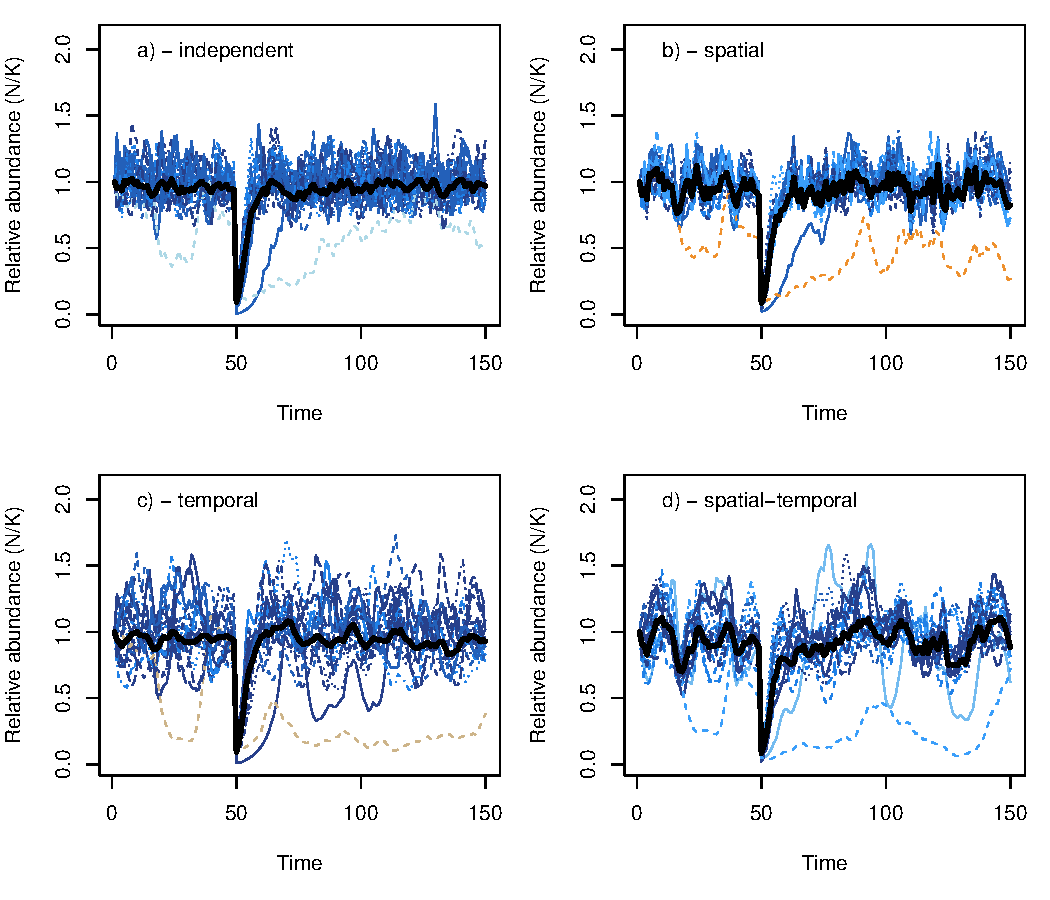
\includegraphics{Managing_for_ecological_surprises_in_metapopulations_files/figure-latex/independent stochasticity-1} 

}

\caption{Metapopulation dynamics with independent (a), spatially correlated (b), temporally correlated (c), and spatio-temporally correlated (d) recruitment deviates.}\label{fig:independent stochasticity}
\end{figure}

\hypertarget{post-disturbance-outcomes}{%
\subsection{Post-disturbance outcomes}\label{post-disturbance-outcomes}}

We measured the following post-disturbance outcomes to track the
temporal and spatial recovery regime of the metapopulation.

\begin{enumerate}
\def\labelenumi{\arabic{enumi}.}
\item
  Recovered (a) \& recovery rate (b) after disturbance:

  \begin{enumerate}
  \def\labelenumii{\alph{enumii}.}
  \tightlist
  \item
    Recovered is defined as the number of simulations where
    metapopulation abundance averaged \texttt{1.0} of the average
    pre-disturbance abundance for \texttt{5} consecutive years
    post-disturbance. This ``recovered rate'' reflects the risk of a
    long-term state shift in metapopulation dynamics after disturbance
    in the face of stochasticity.
  \item
    Recovery rate the number of years to average pre-disturbance
    abundance for \texttt{5} consecutive years. The recovery rate
    (either in the number of generations or in the rate of recovery per
    year) captures how quickly the aggregate metapopulation recovers
    from disturbance but doesn't take into account whether any given
    local patches recover to their pre-disturbance capacity.
  \end{enumerate}
\item
  Patch occupancy - the mean number of patches with
  \texttt{\textgreater{}0.1} local carrying capacity after disturbance
  in the short-term (5 years), medium-term (10 years), and long-term (25
  years). This value characterizes the expected risk of spatial
  contractions or local patch collapses, and reflects how interactions
  between spatial structure, disturbance, and dispersal shape
  source-sink dynamics and the ability to provide (or not) rescue
  effects and recover local patches.
\item
  The ratio of expected maximum surplus production (we term \emph{MSY})
  to true maximum surplus production summed across all patches from
  fitted stock-recruitment model to aggregate across metapopulation such
  that:\\
  \begin{align}
  \Delta_{MSY}=\cfrac{\hat{MSY_M}}{\sum_{i=1}^{N_p} MSY_{i}}
  \end{align}\\
  A value of 1.0 would indicate that the disturbed metapopulation can
  sustain itself against the same disturbance regime as the sum of each
  patch independently. In other words, is the metapopulation more than
  (\(\Delta_{MSY}\)\textgreater{}1.0), less than
  (\(\Delta_{MSY}\)\textless{}1.0), or equal to the sum of its parts
  (\(\Delta_{MSY}\)=1.0).
\end{enumerate}

\hypertarget{monitoring-management-at-aggregate-scale}{%
\subsubsection{Monitoring \& management at
aggregate-scale}\label{monitoring-management-at-aggregate-scale}}

While true metapopulation dynamics are controlled by local patch
dynamics and dispersal such that:

\begin{align}
N_{it}= R_{it}\epsilon_{it}+I_{it}-D_{it}-E_{it}
\end{align}

\begin{align}
R_{it}=\cfrac{\alpha_iN_{it-1}}{1+\cfrac{\alpha_i-1}{\beta_i}N_{it-1}}
\end{align}

\begin{align}
{MN}_t = \sum_{i=1}^{N_p} N_{it}
\end{align}

\begin{align}
{MR}_t = \sum_{i=1}^{N_p} R_{it}
\end{align}

Natural resoure managers often monitors and manages at the scale of the
metapopulation. Hence, management at this scale inherently defines the
stock-recruitment dynamics of the aggregate complex of patches (i.e.,
metapopulation) as:

\begin{align}
{MR}_{t}=\cfrac{\hat{\alpha_t}{MN}_{t-1}}{1+\cfrac{\hat{\alpha_t}-1}{\hat{\beta_t}}{MN}_{it-1}}
\end{align}

where \(\hat{\alpha_t}\) is the estimated compensation ratio averaged
across the metapopulation at time \emph{t} and \(\hat{\beta_t}\) is the
estimated carrying capacity of the entire metapopulation. Necessarily,
these estimates emerge from monitoring data collected across all patches
and are sensitive to the quality of the data and how local patches
perform through time. For example, temporal shifts in productivity
regimes may be masked if most of the data were sampled before the regime
shift. To help surmount these issues, modern resource assessments use
data weighting and penalties (i.e., priors) when fitting models to data.

In our assessment, we weighted recent years of sampling over more
distant years such that:

\begin{figure}[H]

{\centering 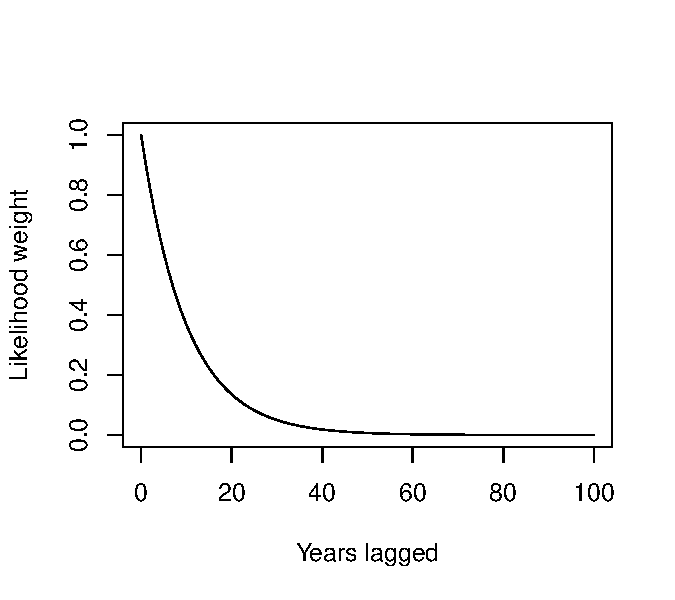
\includegraphics{Managing_for_ecological_surprises_in_metapopulations_files/figure-latex/unnamed-chunk-1-1} 

}

\caption{Likelihood weighting for samples collected over time from current year of sampling.}\label{fig:unnamed-chunk-1}
\end{figure}

This forward-weighting approach increased the sensitivity of the
monitoring sub-model to detect demographic changes in the
post-disturbance recovery regime. Data-weighting is increasingly being
used in resource monitoring, although how weights are developed and
applied to data is a case-by-case basis.

Furthermore, we used penalized normal likelihoods on both
\(\hat{\alpha_t}\) and \(\hat{\beta_t}\) such that:

\begin{align}
\hat{\alpha_t} \sim N(\mu=\hat{\alpha_{t-1}},\sigma=3\hat{\alpha_{t-1}})
\end{align}

and

\begin{align}
\hat{\beta_t} \sim N(\mu=\hat{\beta_{t-1}},\sigma=3\hat{\beta_{t-1}})
\end{align}

where \(\mu=\hat{\alpha_{t-1}}\) and \(\mu=\hat{\beta_{t-1}}\)
represents the best estimates from the previous assessment and the
\texttt{3} in the \(\sigma\) term represents a 300\% coefficient of
variation. We used these penalized likelihoods to fit the above
aggregate stock-recruitment model with \emph{lognormal} error to the
metapopulation stock-recruit data collected at time \emph{t}. We used
the following function and fitted to the below \(\theta\) parameters
(termed \texttt{theta} in the function \texttt{optim()} using the
\texttt{L-BFGS-B} optimizer with a lower bound on \(\hat{\alpha}\) of
\texttt{1.01} (i.e., constrained to be at least above replacement).

\begin{Shaded}
\begin{Highlighting}[]
\NormalTok{SRfn <-}\StringTok{ }\ControlFlowTok{function}\NormalTok{(theta, data, lastYr) \{}
\NormalTok{    a.hat <-}\StringTok{ }\NormalTok{theta[}\DecValTok{1}\NormalTok{]}
\NormalTok{    b.hat <-}\StringTok{ }\KeywordTok{exp}\NormalTok{(theta[}\DecValTok{2}\NormalTok{])}
\NormalTok{    sd.hat <-}\StringTok{ }\KeywordTok{exp}\NormalTok{(theta[}\DecValTok{3}\NormalTok{])}
\NormalTok{    rec.mean <-}\StringTok{ }\NormalTok{(a.hat }\OperatorTok{*}\StringTok{ }\NormalTok{data}\OperatorTok{$}\NormalTok{spawners)}\OperatorTok{/}\NormalTok{(}\DecValTok{1} \OperatorTok{+}\StringTok{ }\NormalTok{((a.hat }\OperatorTok{-}\StringTok{ }\DecValTok{1}\NormalTok{)}\OperatorTok{/}\NormalTok{b.hat) }\OperatorTok{*}\StringTok{ }\NormalTok{data}\OperatorTok{$}\NormalTok{spawners)}
    \CommentTok{# negative log likelihood on recruitment parameters}
\NormalTok{    nll <-}\StringTok{ }\DecValTok{-1} \OperatorTok{*}\StringTok{ }\KeywordTok{sum}\NormalTok{(}\KeywordTok{dlnorm}\NormalTok{(data}\OperatorTok{$}\NormalTok{recruits, }\DataTypeTok{meanlog =} \KeywordTok{log}\NormalTok{(rec.mean), }\DataTypeTok{sdlog =}\NormalTok{ sd.hat, }
        \DataTypeTok{log =} \OtherTok{TRUE}\NormalTok{) }\OperatorTok{*}\StringTok{ }\NormalTok{data}\OperatorTok{$}\NormalTok{weights, }\DataTypeTok{na.rm =} \OtherTok{TRUE}\NormalTok{)}
    \CommentTok{# penalized likelihood on estimated alpha}
\NormalTok{    penalty1 <-}\StringTok{ }\OperatorTok{-}\KeywordTok{dnorm}\NormalTok{(a.hat, lastYr}\OperatorTok{$}\NormalTok{alphaLstYr, }\DecValTok{4} \OperatorTok{*}\StringTok{ }\NormalTok{lastYr}\OperatorTok{$}\NormalTok{alphaLstYr, }\DataTypeTok{log =} \OtherTok{TRUE}\NormalTok{)}
    \CommentTok{# penalized likelihood on estimated carrying capacity}
\NormalTok{    penalty2 <-}\StringTok{ }\OperatorTok{-}\KeywordTok{dnorm}\NormalTok{(b.hat, lastYr}\OperatorTok{$}\NormalTok{metaKLstYr, }\DecValTok{4} \OperatorTok{*}\StringTok{ }\NormalTok{lastYr}\OperatorTok{$}\NormalTok{metaKLstYr, }\DataTypeTok{log =} \OtherTok{TRUE}\NormalTok{)}
\NormalTok{    jnll <-}\StringTok{ }\KeywordTok{sum}\NormalTok{(}\KeywordTok{c}\NormalTok{(nll, penalty1, penalty2), }\DataTypeTok{na.rm =} \OtherTok{TRUE}\NormalTok{)}
    \KeywordTok{return}\NormalTok{(jnll)}
\NormalTok{\}}
\end{Highlighting}
\end{Shaded}

This above function allows us to assess the bias in \(\hat{\alpha_t}\),
\(\hat{\beta_t}\), and \(\hat{MR_t}\) compared to true \(\bar{\alpha}\),
\(\bar{\beta}\), and \({MR}_t\) across the metapopulation. This then
allows us to see how much information management \& monitoring programs
are missing when they assess metapopulations at the aggregate (rather
than local) scales.

\hypertarget{finding-maximum-sustainable-yield}{%
\subsubsection{Finding maximum sustainable
yield}\label{finding-maximum-sustainable-yield}}

Resource managers measure productivity with a variety of performance
reference points (Forrest \emph{et al.} 2010). One of the most widely
used metrics, commonly called \emph{Maximum Sustainable Yield} in
fisheries and other harvest literature (\(MSY\)), relates to the largest
loss the population can sustain over an indefinite period of time while
maximizing its ability to replenish itself. Under density-dependent
growth, individuals' growth, survival, and reproduction at low
population densities are not constrained by limited resources, but
overall production is low because there are few individuals. At high
densities, limited resources increasingly constrain individual's
reproductive success until the population reaches carrying capacity, and
overall production drops to zero because per-capita success is low.
However, at some intermediate densities, both per-capita and overall
production is high, and population growth is at its maximum point due to
the large number of reproducing individuals. At this point, there is the
maximum surplus of individuals produced above replacement that can help
to withstand disturbance or harvest regimes and contribute to future
recovery, either through increasing local patch densities or by
emigrating neighboring patches providing ``rescue effects''.

Under Beverton-Holt or Ricker density-dependent recuitment, however,
there exists no analytical solution for calculating \(MSY\). Therefore,
we used numerical methods and a one dimensional root finder to
iteratively search for the population mortality that maximized surplus
production in the metapopulation. We term this mortality \(F_{MSY}\) and
can use this mortality value to calculate maximum surplus production
\(MSY\), the adult densities that produce \(MSY\) (termed \(N_{MSY}\)),
and the recruits that result from this (termed \(R_{MSY}\)).

\begin{Shaded}
\begin{Highlighting}[]
\CommentTok{# uniroot numerical search}

\NormalTok{yieldRoot <-}\StringTok{ }\ControlFlowTok{function}\NormalTok{(alpha, beta, Fcur, model) \{}
\NormalTok{    Ucur <-}\StringTok{ }\DecValTok{1} \OperatorTok{-}\StringTok{ }\KeywordTok{exp}\NormalTok{(}\OperatorTok{-}\NormalTok{Fcur)}
    \ControlFlowTok{if}\NormalTok{ (model }\OperatorTok{==}\StringTok{ "Beverton-Holt"}\NormalTok{) \{}
        \CommentTok{# population model is R ~ (CR * S)/(1+(CR-1)/K * S): reparameterized}
        \CommentTok{# Beverton-Holt}
\NormalTok{        adults <-}\StringTok{ }\NormalTok{beta }\OperatorTok{*}\StringTok{ }\KeywordTok{exp}\NormalTok{(}\OperatorTok{-}\NormalTok{Fcur)}
\NormalTok{        recruits <-}\StringTok{ }\NormalTok{(alpha }\OperatorTok{*}\StringTok{ }\NormalTok{adults)}\OperatorTok{/}\NormalTok{(}\DecValTok{1} \OperatorTok{+}\StringTok{ }\NormalTok{((alpha }\OperatorTok{-}\StringTok{ }\DecValTok{1}\NormalTok{)}\OperatorTok{/}\NormalTok{beta) }\OperatorTok{*}\StringTok{ }\NormalTok{adults)}
\NormalTok{        yield <-}\StringTok{ }\NormalTok{recruits }\OperatorTok{-}\StringTok{ }\NormalTok{adults}
\NormalTok{    \}}
    \ControlFlowTok{if}\NormalTok{ (model }\OperatorTok{==}\StringTok{ "Ricker"}\NormalTok{) \{}
        \CommentTok{# population model is R ~ CR * S * e(-log(CR)/K * S): reparameterized Ricker}
\NormalTok{        adults <-}\StringTok{ }\NormalTok{beta }\OperatorTok{*}\StringTok{ }\KeywordTok{exp}\NormalTok{(}\OperatorTok{-}\NormalTok{Fcur)}
\NormalTok{        recruits <-}\StringTok{ }\NormalTok{alpha }\OperatorTok{*}\StringTok{ }\NormalTok{adults }\OperatorTok{*}\StringTok{ }\KeywordTok{exp}\NormalTok{((}\OperatorTok{-}\KeywordTok{log}\NormalTok{(alpha)}\OperatorTok{/}\NormalTok{beta) }\OperatorTok{*}\StringTok{ }\NormalTok{adults)}
\NormalTok{        yield <-}\StringTok{ }\NormalTok{recruits }\OperatorTok{-}\StringTok{ }\NormalTok{adults}
\NormalTok{    \}}
    \KeywordTok{return}\NormalTok{(}\KeywordTok{list}\NormalTok{(}\DataTypeTok{recruits =}\NormalTok{ recruits, }\DataTypeTok{adults =}\NormalTok{ adults, }\DataTypeTok{yield =}\NormalTok{ yield))}
\NormalTok{\}}

\CommentTok{# Return approximate gradient for integral}

\NormalTok{fun_yield <-}\StringTok{ }\ControlFlowTok{function}\NormalTok{(Fcur, alpha, beta, delta, model) \{}
\NormalTok{    y1 <-}\StringTok{ }\KeywordTok{yieldRoot}\NormalTok{(}\DataTypeTok{alpha =}\NormalTok{ alpha, }\DataTypeTok{beta =}\NormalTok{ beta, }\DataTypeTok{Fcur =}\NormalTok{ Fcur }\OperatorTok{-}\StringTok{ }\NormalTok{delta}\OperatorTok{/}\DecValTok{2}\NormalTok{, }\DataTypeTok{model =}\NormalTok{ model)}\OperatorTok{$}\NormalTok{yield}
\NormalTok{    y2 <-}\StringTok{ }\KeywordTok{yieldRoot}\NormalTok{(}\DataTypeTok{alpha =}\NormalTok{ alpha, }\DataTypeTok{beta =}\NormalTok{ beta, }\DataTypeTok{Fcur =}\NormalTok{ Fcur }\OperatorTok{+}\StringTok{ }\NormalTok{delta}\OperatorTok{/}\DecValTok{2}\NormalTok{, }\DataTypeTok{model =}\NormalTok{ model)}\OperatorTok{$}\NormalTok{yield}
\NormalTok{    approx.gradient <-}\StringTok{ }\NormalTok{(y2 }\OperatorTok{-}\StringTok{ }\NormalTok{y1)}\OperatorTok{/}\NormalTok{delta}
    \KeywordTok{return}\NormalTok{(approx.gradient)}
\NormalTok{\}}

\CommentTok{# uniroot search for optimal yield and Fmsy}
\NormalTok{findMSY <-}\StringTok{ }\ControlFlowTok{function}\NormalTok{(alpha, beta, Npatches, model) \{}
\NormalTok{    F_msy <-}\StringTok{ }\OtherTok{NULL}
    \ControlFlowTok{for}\NormalTok{ (i }\ControlFlowTok{in} \DecValTok{1}\OperatorTok{:}\NormalTok{Npatches) \{}
\NormalTok{        a_p <-}\StringTok{ }\NormalTok{alpha[i]}
\NormalTok{        b_p <-}\StringTok{ }\NormalTok{beta[i]}
\NormalTok{        F_msy[i] <-}\StringTok{ }\KeywordTok{uniroot}\NormalTok{(fun_yield, }\DataTypeTok{interval =} \KeywordTok{c}\NormalTok{(}\DecValTok{0}\NormalTok{, }\DecValTok{1}\NormalTok{), }\DataTypeTok{extendInt =} \StringTok{"yes"}\NormalTok{, }
            \DataTypeTok{alpha =}\NormalTok{ a_p, }\DataTypeTok{beta =}\NormalTok{ b_p, }\DataTypeTok{delta =} \FloatTok{1e-04}\NormalTok{, }\DataTypeTok{model =}\NormalTok{ model)}\OperatorTok{$}\NormalTok{root}
\NormalTok{    \}}
\NormalTok{    MSY <-}\StringTok{ }\KeywordTok{sapply}\NormalTok{(}\DecValTok{1}\OperatorTok{:}\NormalTok{Npatches, }\ControlFlowTok{function}\NormalTok{(x) \{}
        \KeywordTok{yieldRoot}\NormalTok{(}\DataTypeTok{alpha =}\NormalTok{ alpha[x], }\DataTypeTok{beta =}\NormalTok{ beta[x], }\DataTypeTok{Fcur =}\NormalTok{ F_msy[[x]][}\DecValTok{1}\NormalTok{], }\DataTypeTok{model =}\NormalTok{ model)}
\NormalTok{    \})}
    \KeywordTok{return}\NormalTok{(}\KeywordTok{list}\NormalTok{(}\DataTypeTok{F_msy =}\NormalTok{ F_msy, }\DataTypeTok{MSY =}\NormalTok{ MSY))}
\NormalTok{\}}
\end{Highlighting}
\end{Shaded}

\hypertarget{scenarios}{%
\subsection{Scenarios}\label{scenarios}}

We tested all combinations of the following eight processes (below) and
ran a \texttt{100} bootstraps per scenario to estimate the mean for each
of the above outcomes.

\begin{enumerate}
\def\labelenumi{\arabic{enumi}.}
\item
  Homogenous and spatially variable recruitment compensation ratio
  across patches, i.e.~intrinsic rate of population growth
  (\(\alpha_i\)).
\item
  Homogenous and spatially variable local carrying capacity across
  patches, i.e.~asymptote of expected recruits at high adult densities
  (\(\beta_i\))
\item
  Disturbances where a proportion of individuals removed from
  metapopulation (e.g., \texttt{0.90}) occurs.

  \begin{enumerate}
  \def\labelenumii{\alph{enumii}.}
  \tightlist
  \item
    \emph{uniform} - random individuals removed at equal vulnerability
    across all patches.
  \item
    \emph{localized, random} - random individuals removed from randomly
    selected subset of patches (as long as the target individuals lost
    in the metapopulation can be achieved in that subset of patches)
  \item
    \emph{localized, extirpation} - total extirpation of randomly
    selected subset of patches (as long as the target individuals lost
    in the metapopulation can be achieved in that subset of patches)
  \end{enumerate}
\item
  Density-independent dispersal rates \(\omega\) from 0 to 20\% of
  individuals within a patch will disperse.
\item
  Topology of the spatial networks with linear, dendritic, star, and
  complex networks. Each network with \(N_p\) of \texttt{16} and
  distance between patches \(\bar{d}\) of \texttt{1}.
\item
  Stochastic recruitment deviates from low, medium, high coefficient of
  variation on lognormal error. Generate stochasticity in time-dynamics
  via random recruitement deviates away from expected.
\item
  Temporal correlation in recruitment deviates from low, medium, high
  correlation (i.e., good year at time \emph{t} begets good year at time
  \emph{t+1}).
\item
  Spatial correlation in recruitment deviates among patches from low,
  medium, to high correlation (i.e., neighboring patches go up or down
  together).
\end{enumerate}

\hypertarget{example-results}{%
\subsubsection{Example results}\label{example-results}}

We demonstrate our metapopulation model with an example outcome for a
linear network composed of \texttt{16} patches, a dispersal rate of
\texttt{0.01} and a high enough dispersal cost such that individuals are
only willing to move to their closest neighboring patches. This limits
the strength of potential rescue effects. For this example, patches
varied in their productivity and carrying capacity but will have
deterministic population dynamics.

\begin{figure}[H]

{\centering 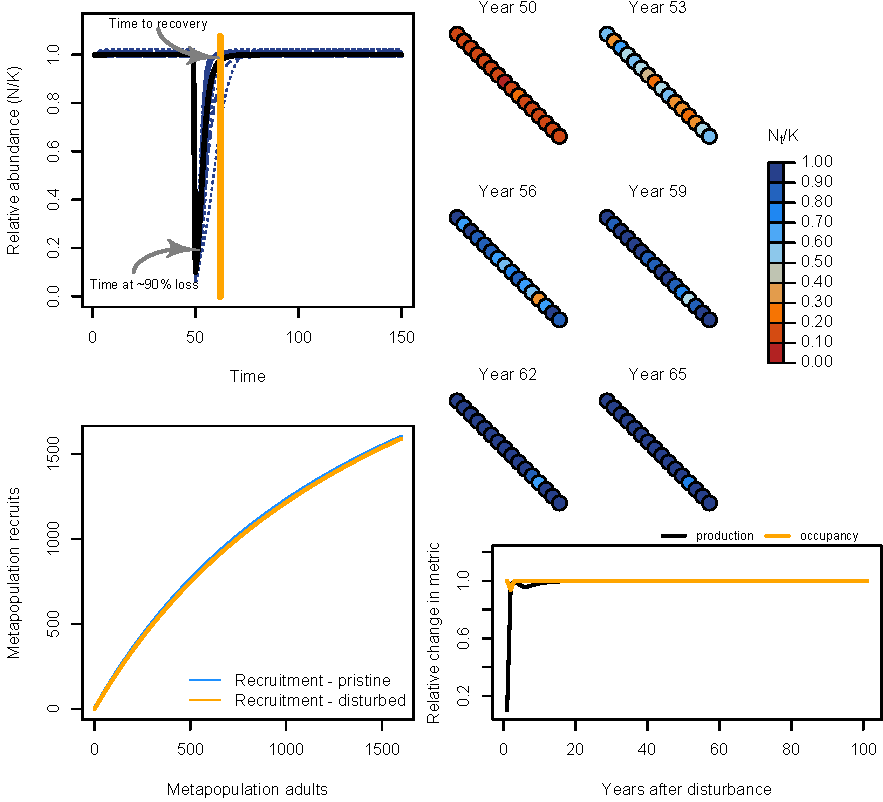
\includegraphics{Managing_for_ecological_surprises_in_metapopulations_files/figure-latex/example results1-1} 

}

\caption{Spatial recovery regime of metapopulation with linear topology through time (top left) and space (top right). Recruitment dynamics before and 10 years after disturbance (bottom left). Relative bias in aggregate-scale estimates of carrying capacity, compensation ratio, and recruitment production in recovery phase (bottom right).}\label{fig:example results1}
\end{figure}
\newpage

We can then contrast this with a different network shape, like a
dendritic network.

\begin{figure}[H]

{\centering 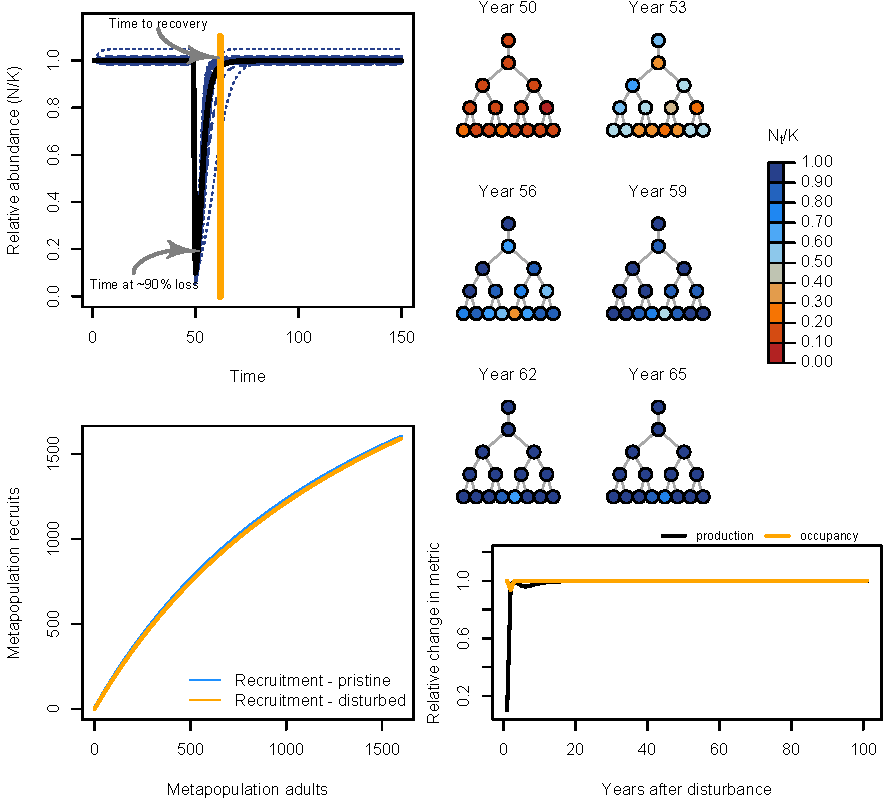
\includegraphics{Managing_for_ecological_surprises_in_metapopulations_files/figure-latex/example results2-1} 

}

\caption{Spatial recovery regime of metapopulation with dendritic topology.}\label{fig:example results2}
\end{figure}
\newpage

Now, let's add some stochasticity to recruitment and see how this
affects the recovery regime.

\begin{figure}[H]

{\centering 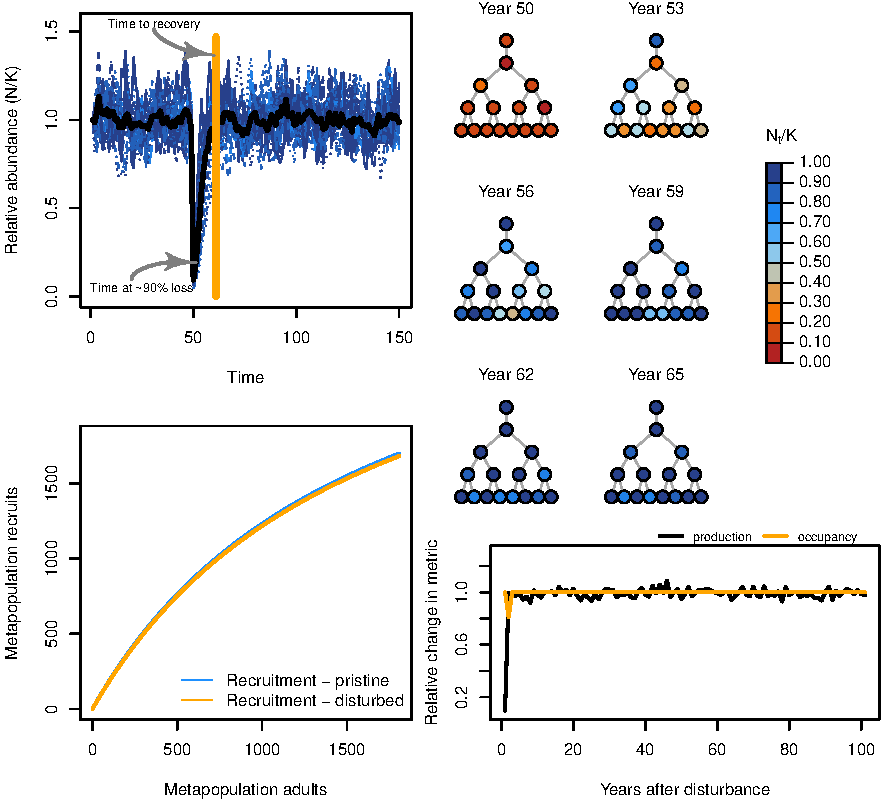
\includegraphics{Managing_for_ecological_surprises_in_metapopulations_files/figure-latex/example results3-1} 

}

\caption{Spatial recovery regime of stochastic metapopulation.}\label{fig:example results3}
\end{figure}
\newpage

Next, we can contrast with a disturbance regime where the disturbance is
concentrated on local patches that can be completely extirpated (rather
than the disturbance being applied proportionally across all patches
e.g., a mixed-stock fishery).

\begin{figure}[H]

{\centering 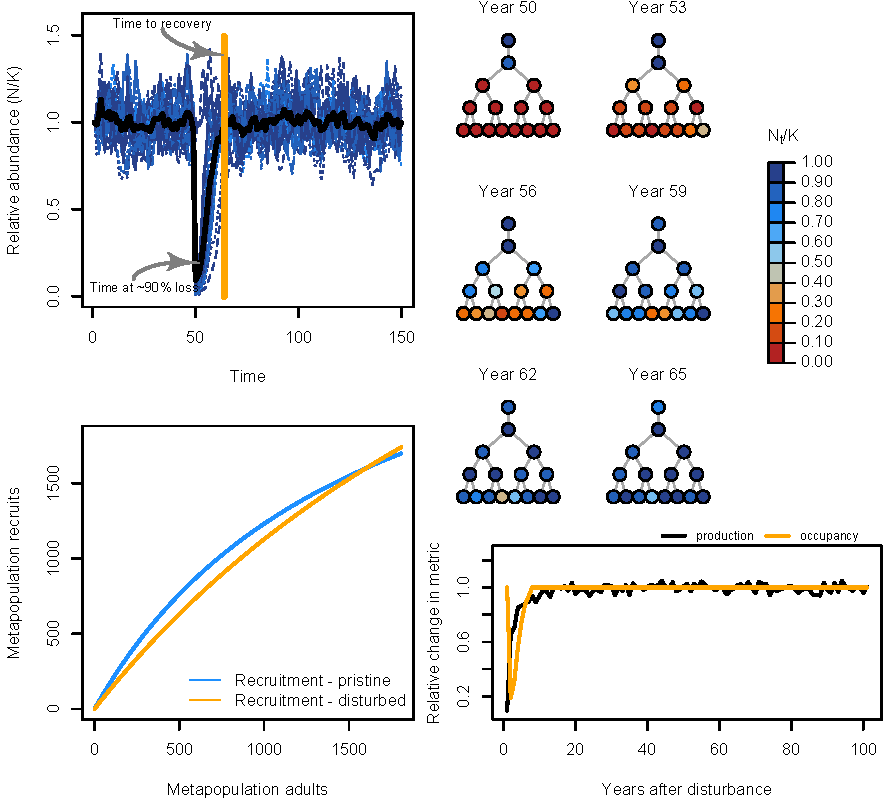
\includegraphics{Managing_for_ecological_surprises_in_metapopulations_files/figure-latex/example results4-1} 

}

\caption{Spatial recovery regime of stochastic metapopulation.}\label{fig:example results4}
\end{figure}
\newpage

\hypertarget{general-patterns}{%
\subsection{General patterns}\label{general-patterns}}

\hypertarget{effects-of-disturbance-regime}{%
\subsubsection{Effects of disturbance
regime}\label{effects-of-disturbance-regime}}

\begin{figure}[H]

{\centering 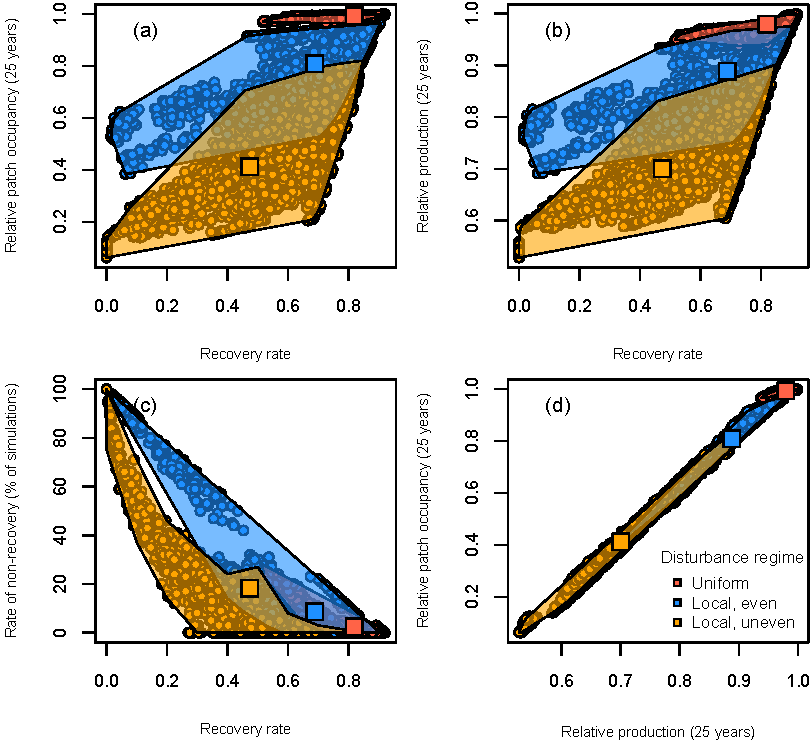
\includegraphics{Managing_for_ecological_surprises_in_metapopulations_files/figure-latex/disturbance regime-1} 

}

\caption{Spatial and temporal recovery patterns along disturbance regimes.}\label{fig:disturbance regime}
\end{figure}

\hypertarget{role-of-network-structure-dispersal}{%
\subsubsection{Role of network structure \&
dispersal}\label{role-of-network-structure-dispersal}}

We now show some general patterns in how variable patch demographic
rates, network structure, dispersal, disturbance, recruitment
stochasticity, and spatio-temporal correlations variation affects
metapopulation \emph{recovery rates}, \emph{maximum sustainable yield}
(analagous to the maximum rate of loss the system can sustain), and
\emph{recovered} (i.e, the number of simulations where the
metapopulation fails to recover), and \emph{patch occupancy} (i.e.,
number of patches with local abundance above some baseline).

First, lets show recovery rates for a scenario where (1) patches have
the same local productivities and carrying capacities, (2) patches have
different productivities and carrying capacities, (3) recruitment is
deterministic and patches are different, and (4) spatial-temporal
correlation in stochastic recruitment.

Below, we can see three main effects on recovery rates (number of
generations to reach recovery). First, recovery gets faster with
increased dispersal. Most of the action here takes place at low rates of
dispersal indicating most spatial topologies don't need much dispersal
to quicken their recovery. In preliminary runs, dispersal rates of
\texttt{0.05-0.2} provided similar recovery patterns. Second, more
localized disturbances regimes lead to slower recovery. Third,
linearized networks have slower recovery times than interconnected,
complex networks suggesting that rescue effects take some time to
cascade through the entire network of patches.

\begin{figure}[H]

{\centering 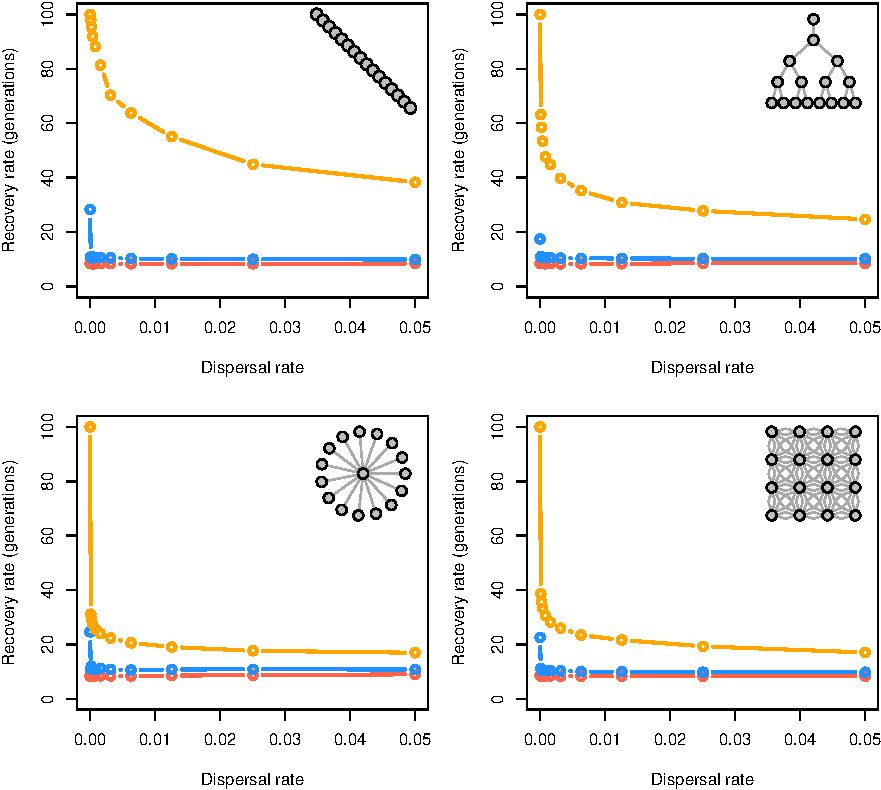
\includegraphics{Managing_for_ecological_surprises_in_metapopulations_files/figure-latex/general results-1} 

}

\caption{Recovery rates along dispersal, disturbance (red - uniform; blue - localized, random; orange - localized, extirpation), and network gradients without stochasticity.}\label{fig:general results}
\end{figure}
\newpage

Now, lets show recovery rates for the same scenario with deterministic
recruitment but allowing for patches to vary in productivity and
carrying capacity. In addition to the same three main effects of
dispersal, network, and disturbance noted above, we also see variable
patch productivities slows recovery across all scenarios.

\begin{figure}[H]

{\centering 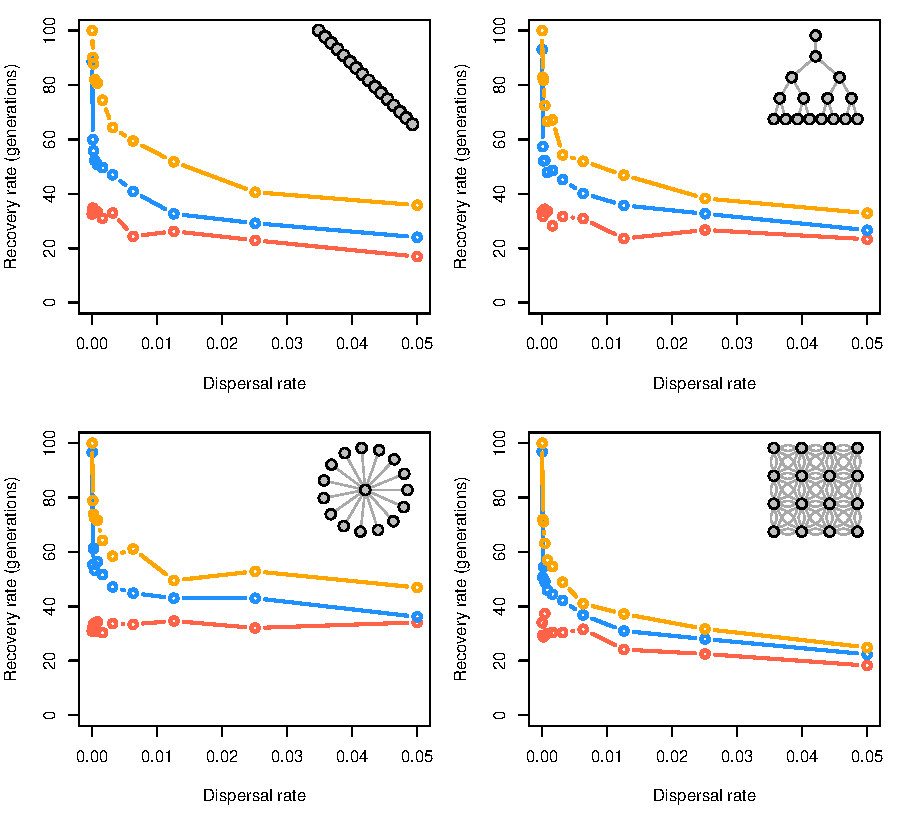
\includegraphics{Managing_for_ecological_surprises_in_metapopulations_files/figure-latex/results for variables patches-1} 

}

\caption{Recovery rates along dispersal, disturbance (red - uniform; blue - localized, random; orange - localized, extirpation), and network gradients with variable local productivity and carrying capacities.}\label{fig:results for variables patches}
\end{figure}
\newpage

Now, lets show recovery rates for the same scenario but allowing for
recruitment to be stochastic (but patches are the same in demography).
We see the same three main effects of dispersal, network, and
disturbance noted above. We also see a few subtle changes: (1)
stochasticity slows recovery for uniform and local disturbance, but (2)
quickens recovery for extreme local disturbance.

\begin{figure}[H]

{\centering 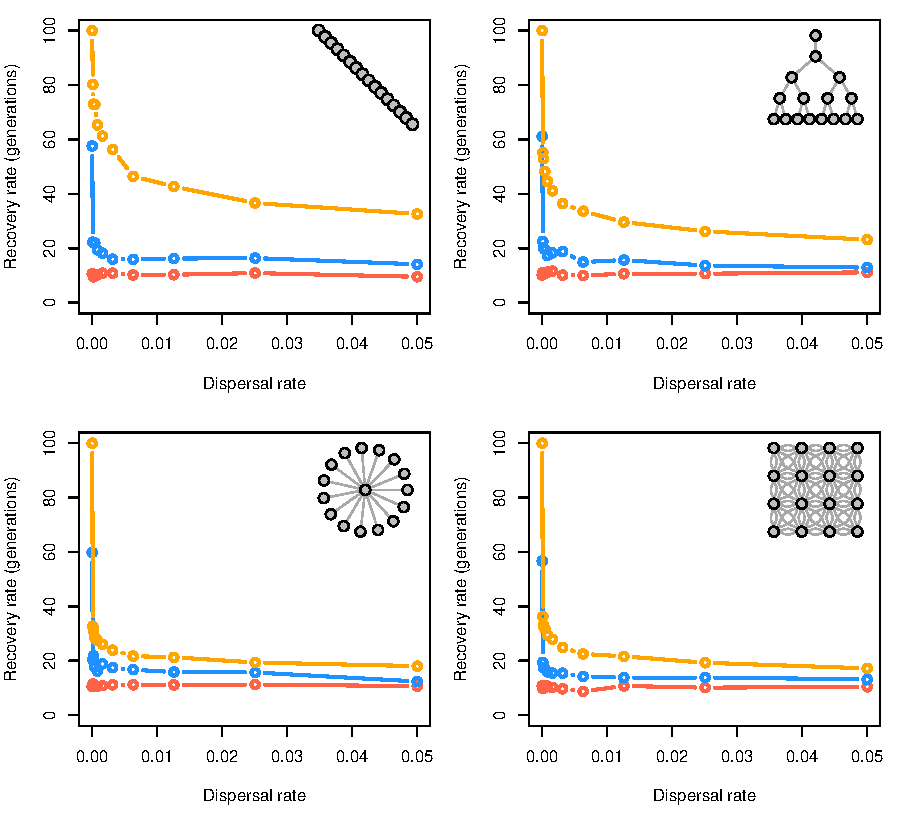
\includegraphics{Managing_for_ecological_surprises_in_metapopulations_files/figure-latex/stochastic recruitment-1} 

}

\caption{Recovery rates along dispersal, disturbance (red - uniform; blue - localized, random; orange - localized, extirpation), and network gradients with stochasticity.}\label{fig:stochastic recruitment}
\end{figure}
\newpage

Now, lets show recovery rates for the same scenarios but with spatial
and temporal correlations in recruitment stochasticity. In addition to
the same effects of stochasticity, we also generally see a small effect
of slower recovery times for uniform and local disturbance, but faster
recovery times for extreme localized disturbance.

\begin{figure}[H]

{\centering 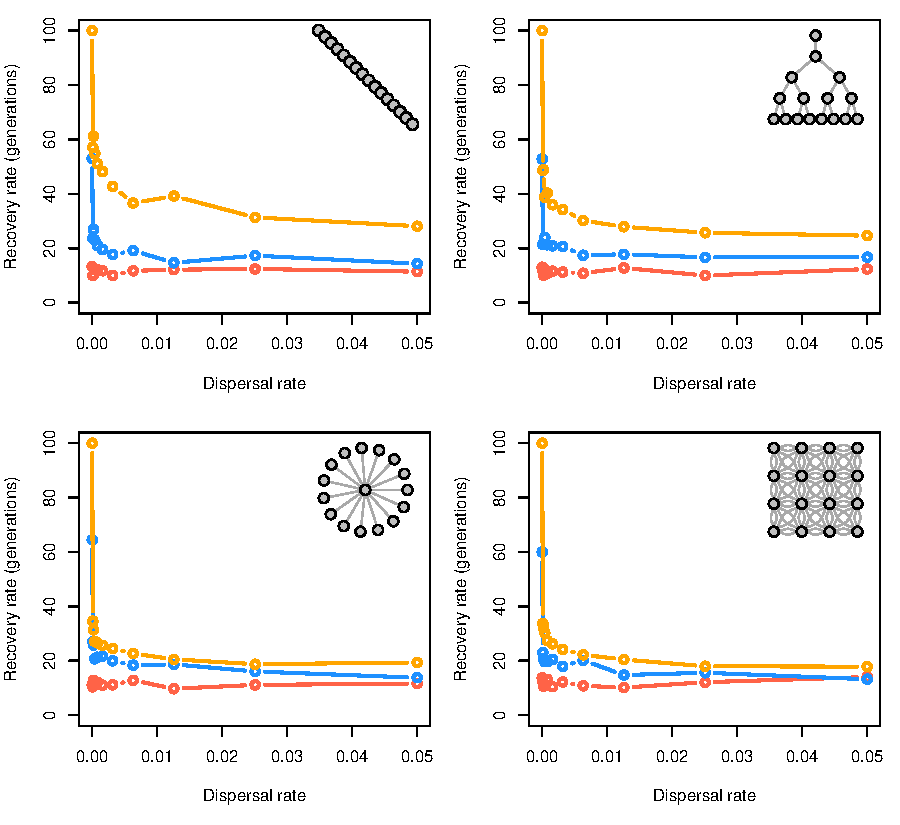
\includegraphics{Managing_for_ecological_surprises_in_metapopulations_files/figure-latex/spatiotemporal correlation-1} 

}

\caption{Recovery rates along dispersal, disturbance (red - uniform; blue - localized, random; orange - localized, extirpation), and network gradients with high spatial-temporal correlation in recruitment variation.}\label{fig:spatiotemporal correlation}
\end{figure}
\newpage

\hypertarget{general-patterns-in-msy}{%
\subsubsection{General patterns in MSY}\label{general-patterns-in-msy}}

\hypertarget{msy-with-deterministic-recruitment-where-patches-are-the-same}{%
\paragraph{MSY with deterministic recruitment where patches are the
same}\label{msy-with-deterministic-recruitment-where-patches-are-the-same}}

We now show similar patterns in how the maximum surplus production of
the whole metapopulation (i.e., MSY) shifts in the first 25 years
post-disturbance compared to the sum of MSY for each patch. A value of
1.0 would indicate that the disturbed metapopulation can sustain itself
against the same disturbance regime as the sum of each patch
independently. In other words, is the metapopulation more, less, or
equal to the sum of its parts.

We will show 25-year MSY patterns for a scenario where (1) patches have
the same local productivities and carrying capacities, (2) patches have
different productivities and carrying capacities, (3) recruitment is
deterministic and patches are different, (4) spatial-temporal
correlation in stochastic recruitment.

Below, we can see three main effects on recovery rates (number of
generations to reach recovery). First, recovery gets faster with
increased dispersal. Most of the action here takes place at low rates of
dispersal indicating most spatial topologies don't need much dispersal
to quicken their recovery. In preliminary runs, dispersal rates of
\texttt{0.05-0.2} provided similar recovery patterns. Second, more
localized disturbances regimes lead to slower recovery. Third,
linearized networks have slower recovery times than interconnected,
complex networks suggesting that rescue effects take some time to
cascade through the entire network of patches.

\begin{figure}[H]

{\centering 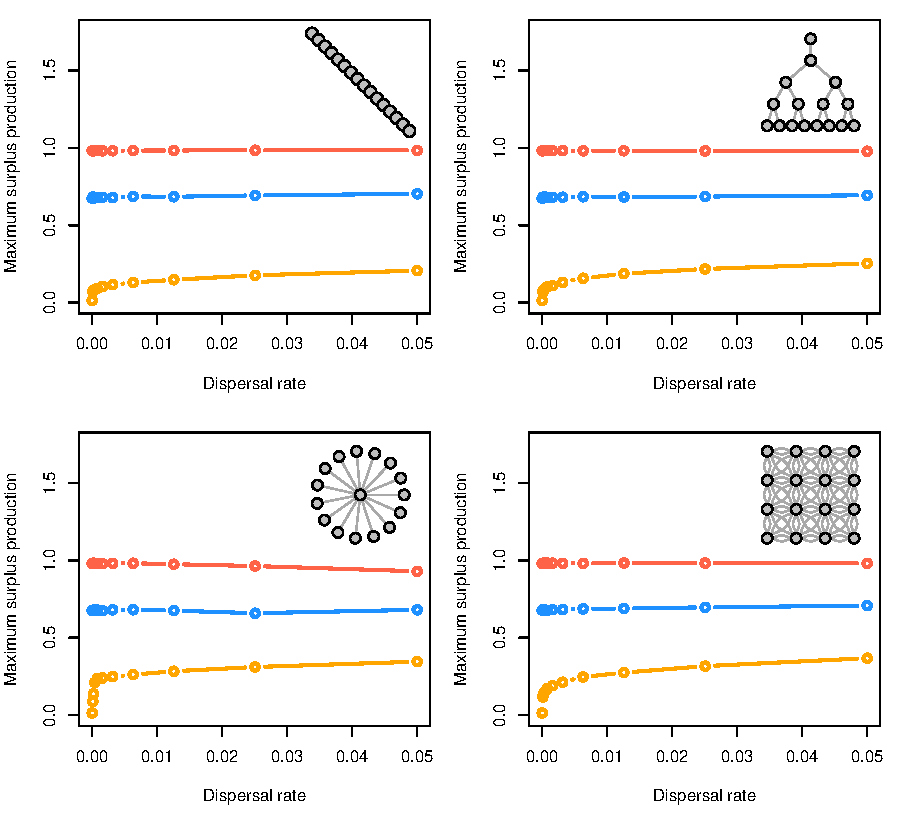
\includegraphics{Managing_for_ecological_surprises_in_metapopulations_files/figure-latex/MSY-1} 

}

\caption{Maximum surplus production along dispersal, disturbance (red - uniform; blue - localized, random; orange - localized, extirpation), and network gradients with deterministic recruitment and the same patches.}\label{fig:MSY}
\end{figure}

\newpage

\hypertarget{msy-with-variable-patches}{%
\paragraph{MSY with variable patches}\label{msy-with-variable-patches}}

Now, we illustrate how variable patch demography affects the 25-year
average MSY.

\begin{figure}[H]

{\centering 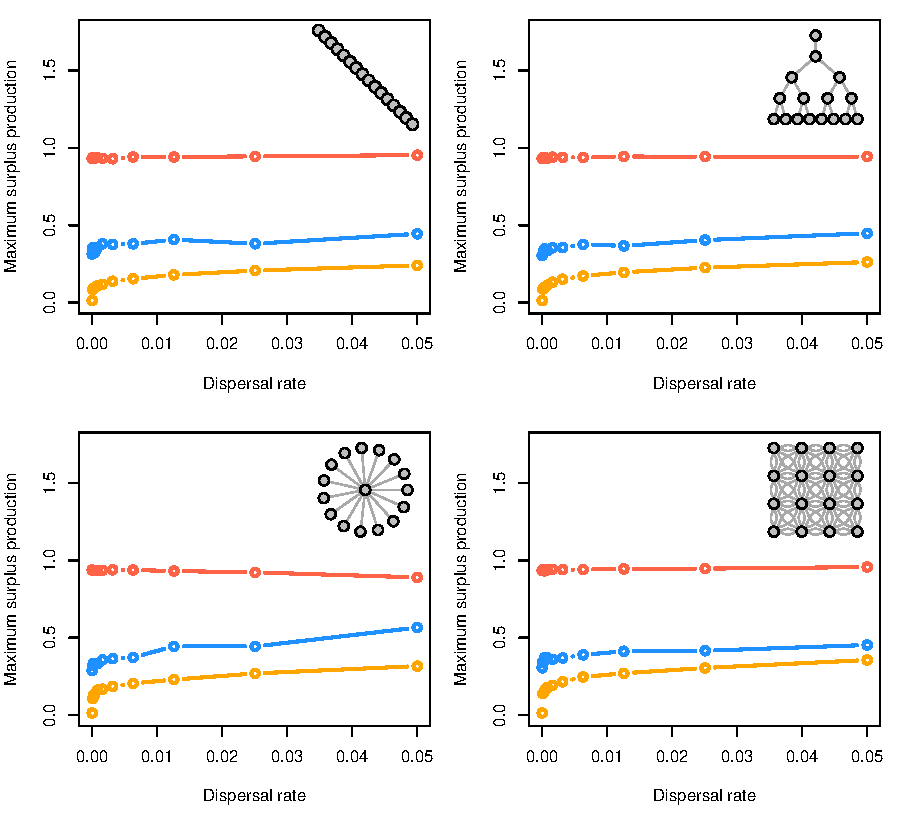
\includegraphics{Managing_for_ecological_surprises_in_metapopulations_files/figure-latex/MSY with variable patches-1} 

}

\caption{Maximum surplus production along dispersal, disturbance (red - uniform; blue - localized, random; orange - localized, extirpation), and network gradients with variable patches.}\label{fig:MSY with variable patches}
\end{figure}
\newpage

\hypertarget{msy-with-variable-patches-and-stochasticity}{%
\paragraph{MSY with variable patches and
stochasticity}\label{msy-with-variable-patches-and-stochasticity}}

Now, we illustrate how variable patch demography affects the 25-year
average MSY.

\begin{figure}[H]

{\centering 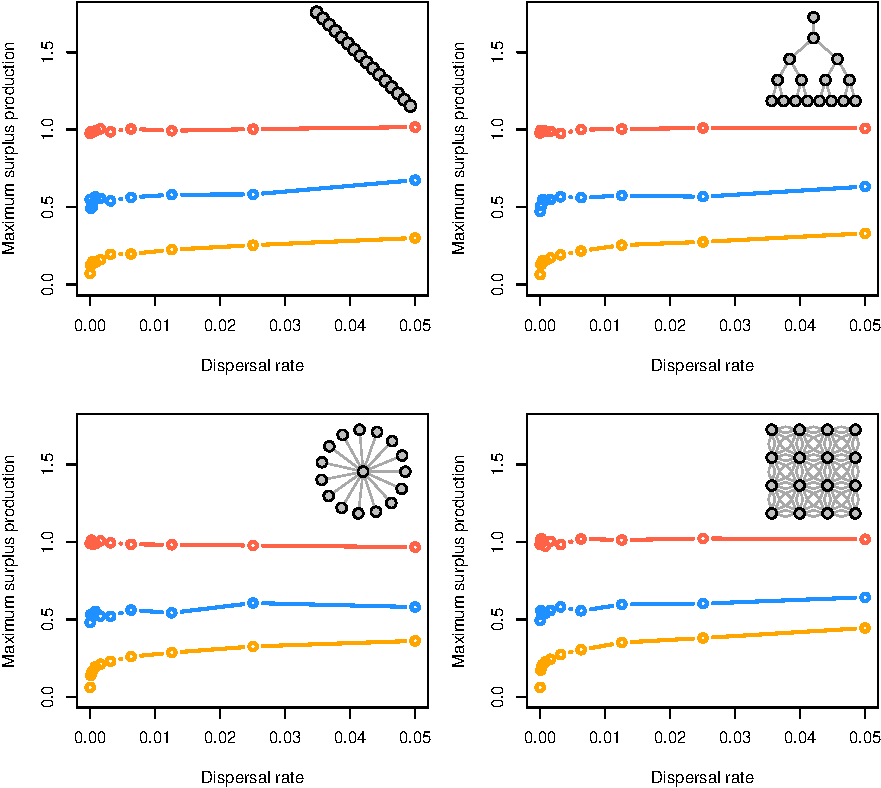
\includegraphics{Managing_for_ecological_surprises_in_metapopulations_files/figure-latex/MSY with variable patches and stochasticity-1} 

}

\caption{Maximum surplus production along dispersal, disturbance (red - uniform; blue - localized, random; orange - localized, extirpation), and network gradients with variable patches and stochasticity.}\label{fig:MSY with variable patches and stochasticity}
\end{figure}
\newpage

\hypertarget{msy-with-variable-patches-and-spatio-temporally-correlated-stochasticity}{%
\paragraph{MSY with variable patches, and spatio-temporally correlated
stochasticity}\label{msy-with-variable-patches-and-spatio-temporally-correlated-stochasticity}}

Now, we illustrate how variable patch demography and high
spatial-temporal correlations in stochastic recruitment affects the
25-year average MSY.

\begin{figure}[H]

{\centering 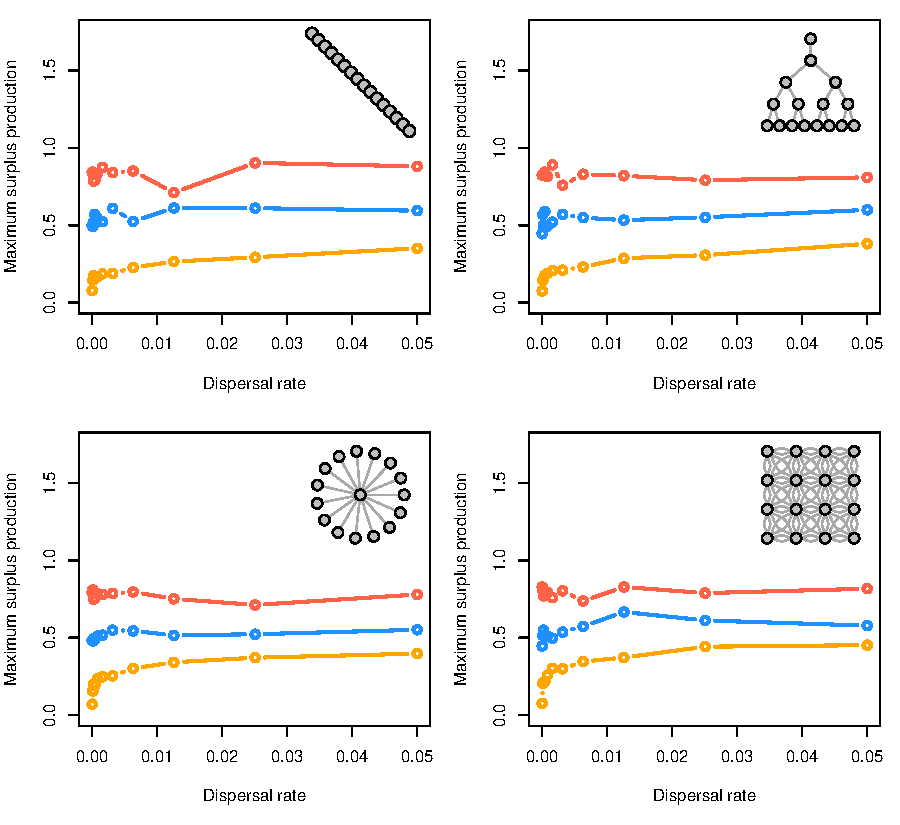
\includegraphics{Managing_for_ecological_surprises_in_metapopulations_files/figure-latex/MSY with variable patches and space-time stochasticity-1} 

}

\caption{Maximum surplus production along dispersal, disturbance (red - uniform; blue - localized, random; orange - localized, extirpation), and network gradients with high spatial-temporal correlation in recruitment stochasticity and variable patches.}\label{fig:MSY with variable patches and space-time stochasticity}
\end{figure}

\newpage

\hypertarget{general-patterns-in-the-risk-of-hysteresis-state-shifts}{%
\subsubsection{General patterns in the risk of hysteresis \& state
shifts}\label{general-patterns-in-the-risk-of-hysteresis-state-shifts}}

We now show similar patterns in the lack of recovery across the
metapopulation after \(100\) generations post-disturbance. Recovered \%
is defined as the number of simulations where metapopulation abundance
averaged \texttt{1.0} of the average pre-disturbance abundance for
\texttt{5} consecutive years after disturbance. This ``recovered rate''
reflects the risk of a long-term state shift in metapopulation dynamics
after disturbance in the face of stochasticity. We start with a scenario
with deterministic recruitment where patches are the same.

\begin{figure}[H]

{\centering 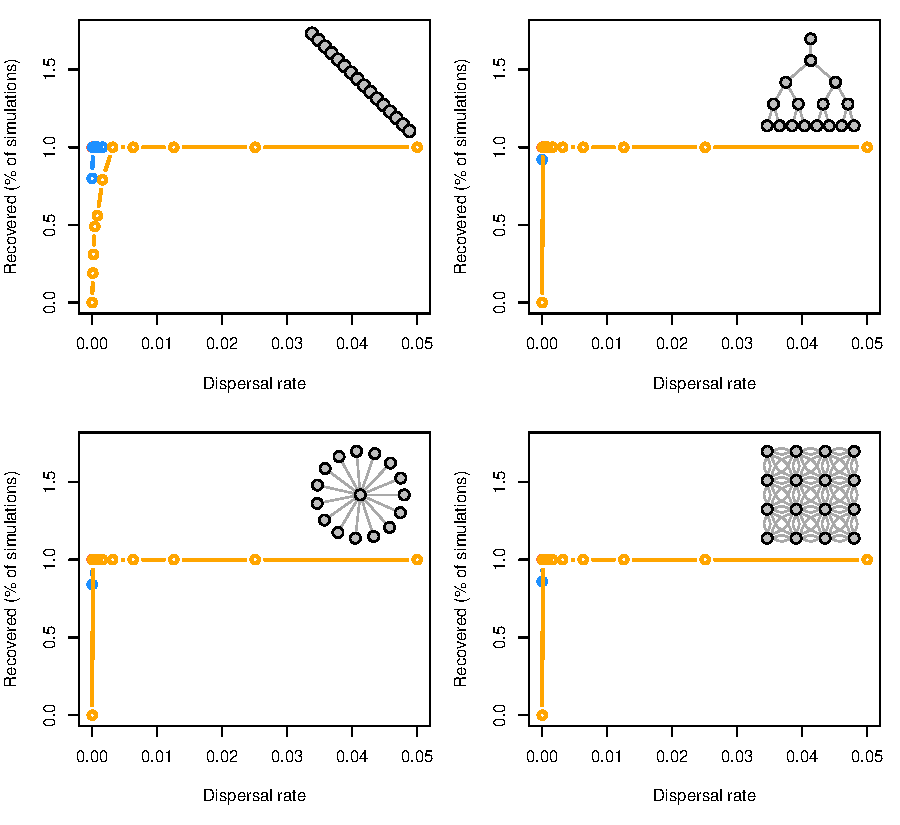
\includegraphics{Managing_for_ecological_surprises_in_metapopulations_files/figure-latex/Recovery-1} 

}

\caption{Risk of state shift after 100 generations along dispersal, disturbance (red - uniform; blue - localized, random; orange - localized, extirpation), and network gradients with high spatial-temporal correlation in recruitment variation.}\label{fig:Recovery}
\end{figure}
\newpage

\hypertarget{state-shifts-with-variable-patches}{%
\paragraph{State shifts with variable
patches}\label{state-shifts-with-variable-patches}}

Now, we illustrate how variable patch demography affects the risk of a
state shift.

\begin{figure}[H]

{\centering 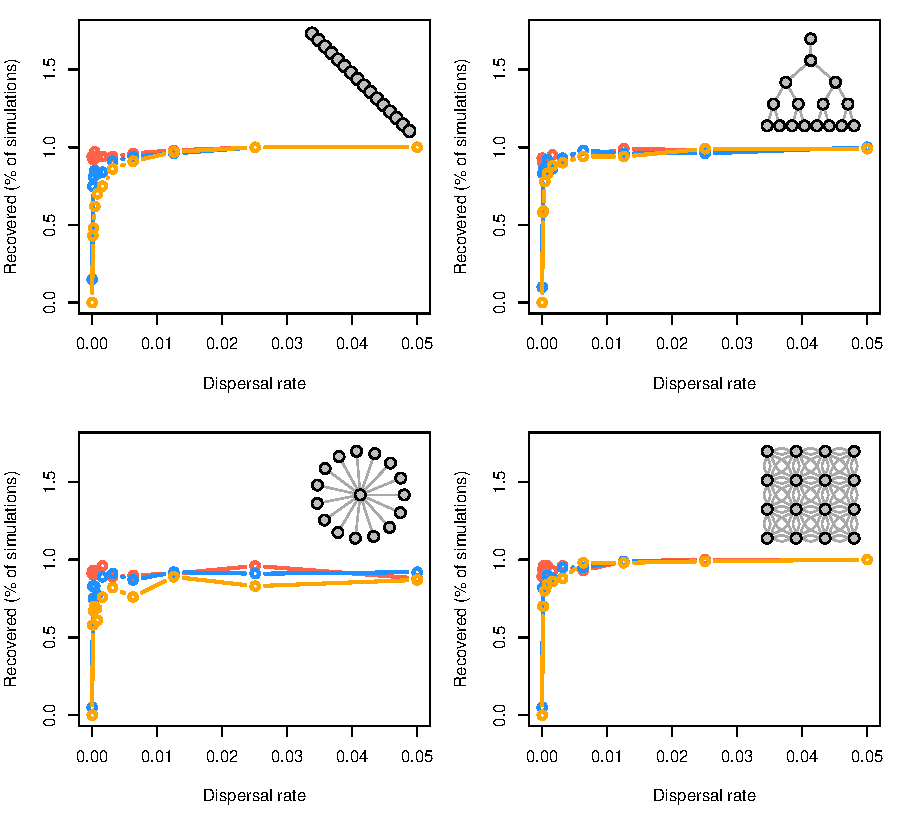
\includegraphics{Managing_for_ecological_surprises_in_metapopulations_files/figure-latex/unrecovered with variable patches-1} 

}

\caption{Risk of state shift after 100 generations along dispersal, disturbance (red - uniform; blue - localized, random; orange - localized, extirpation), and network gradients with variable patches.}\label{fig:unrecovered with variable patches}
\end{figure}
\newpage

\hypertarget{state-shifts-with-variable-patches-and-stochasticity}{%
\paragraph{State shifts with variable patches and
stochasticity}\label{state-shifts-with-variable-patches-and-stochasticity}}

Now, we illustrate how variable patch demography and stochastic
recruitment affects the risk of state shift.

\begin{figure}[H]

{\centering 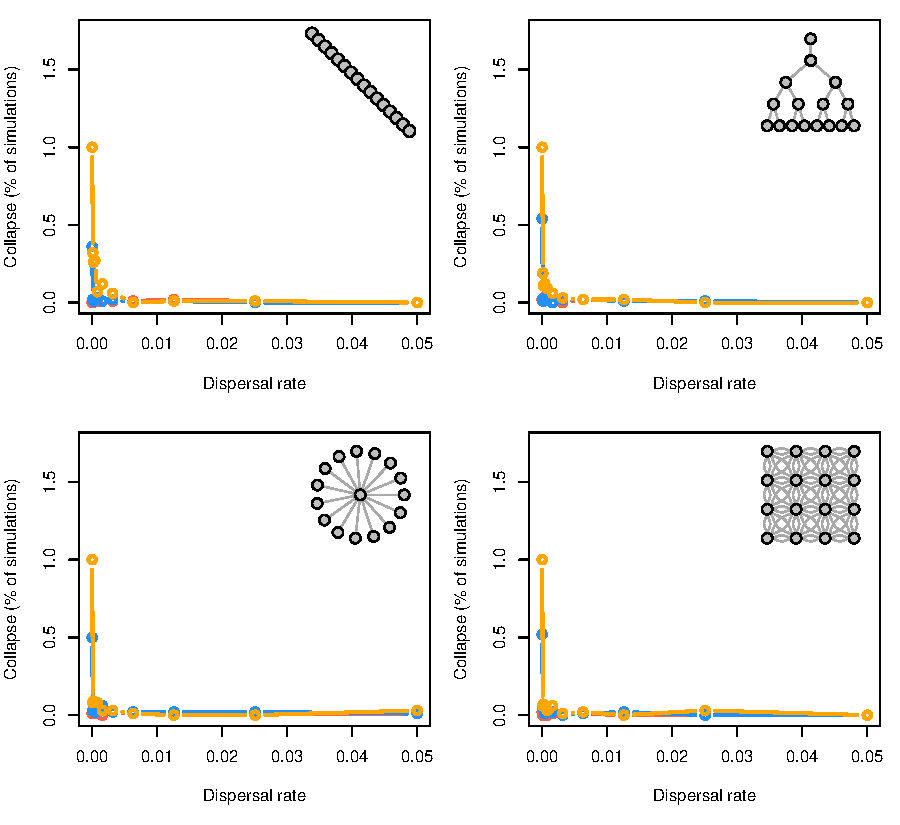
\includegraphics{Managing_for_ecological_surprises_in_metapopulations_files/figure-latex/state shift with variable patches and stochasticity-1} 

}

\caption{Risk of state shift after 100 generations along dispersal, disturbance (red - uniform; blue - localized, random; orange - localized, extirpation), and network gradients with variable patches and stochastic recruitment.}\label{fig:state shift with variable patches and stochasticity}
\end{figure}
\newpage

\hypertarget{state-shifts-with-variable-patches-and-spatio-temporally-correlated-stochasticity}{%
\paragraph{State shifts with variable patches, and spatio-temporally
correlated
stochasticity}\label{state-shifts-with-variable-patches-and-spatio-temporally-correlated-stochasticity}}

Now, we illustrate how variable patch demography and high
spatial-temporal correlations in stochastic recruitment affects the risk
of a state shift.

\begin{figure}[H]

{\centering 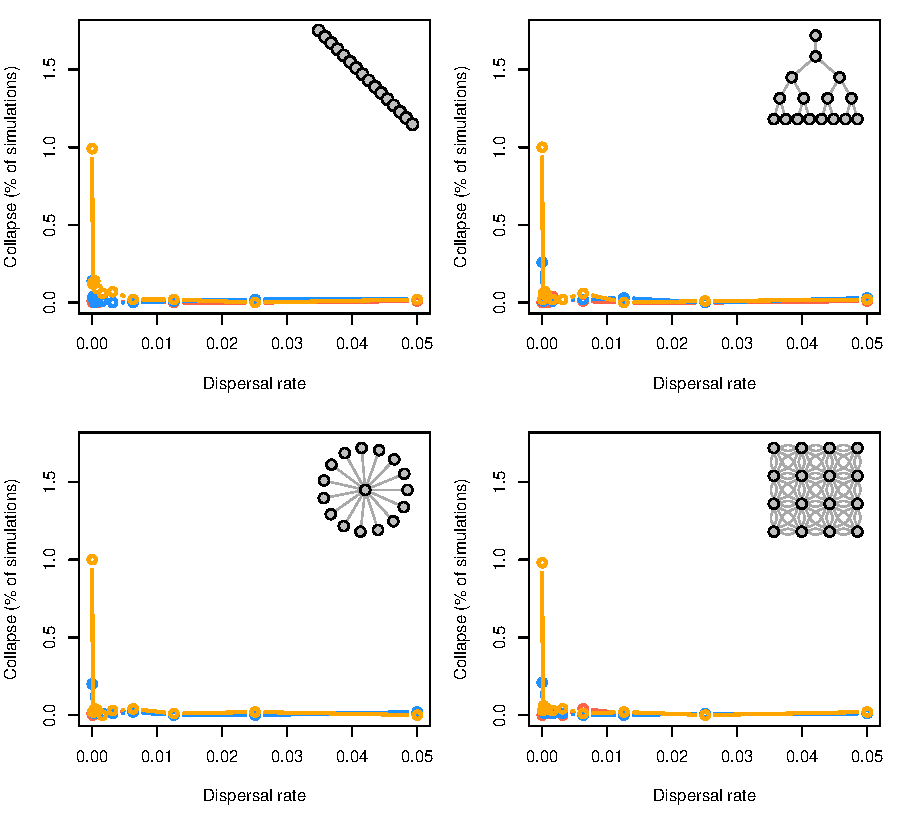
\includegraphics{Managing_for_ecological_surprises_in_metapopulations_files/figure-latex/state shifts with variable patches and space-time stochasticity-1} 

}

\caption{Risk of state shift (lack of recovery or spatial contraction) after 100 generations along dispersal, disturbance (red - uniform; blue - localized, random; orange - localized, extirpation), and network gradients with variable patches, and spatial-temporal correlations in stochastic recruitment.}\label{fig:state shifts with variable patches and space-time stochasticity}
\end{figure}

\newpage

\hypertarget{general-patterns-in-the-risk-of-spatial-contraction}{%
\subsubsection{General patterns in the risk of spatial
contraction}\label{general-patterns-in-the-risk-of-spatial-contraction}}

We now show similar patterns in patch occupancy after \(25\) years
post-disturbance. Patch occupancy is defined as the average number of
patches that fail to recover above \texttt{0.1} pre-disturbance
abundance for scenario with deterministic recruitment where patches are
the same. Patch occupancy characterizes the expected risk of spatial
contractions or local patch collapses, and reflects how interactions
between spatial structure, disturbance, and dispersal affect source-sink
dynamics and the provisioning of rescue effects to local patches.

\begin{figure}[H]

{\centering 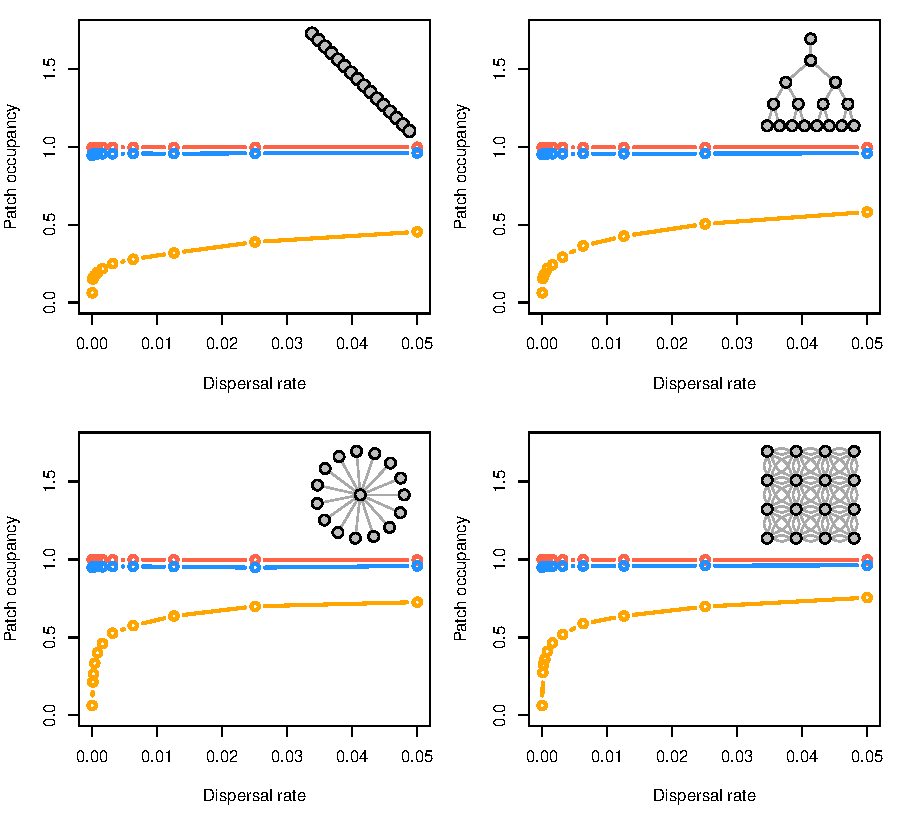
\includegraphics{Managing_for_ecological_surprises_in_metapopulations_files/figure-latex/patch occupancy-1} 

}

\caption{Patch occupancy after 25 years along dispersal, disturbance (red - uniform; blue - localized, random; orange - localized, extirpation), and network gradients with deterministic recruitment and homogeouns patches.}\label{fig:patch occupancy}
\end{figure}
\newpage

\hypertarget{patch-occupancy-with-variable-patches}{%
\paragraph{Patch occupancy with variable
patches}\label{patch-occupancy-with-variable-patches}}

Now, we illustrate how variable patch demography affects patch
occupancy.

\begin{figure}[H]

{\centering 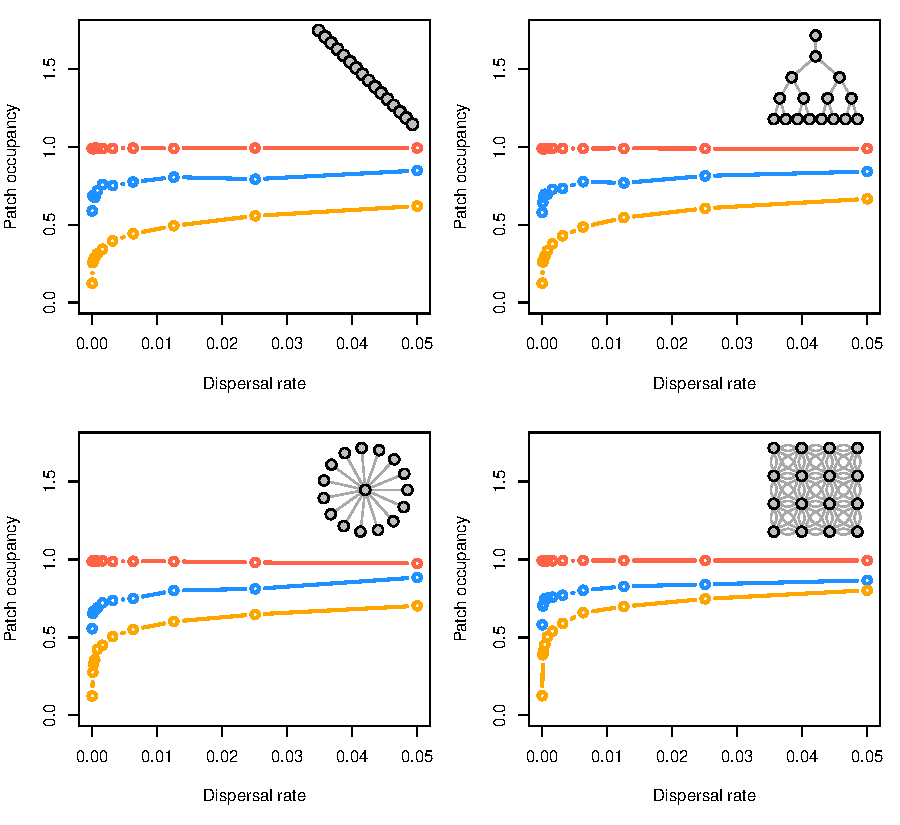
\includegraphics{Managing_for_ecological_surprises_in_metapopulations_files/figure-latex/patch occupancy with variable patches-1} 

}

\caption{Patch occupancy after 25 years along  dispersal, disturbance (red - uniform; blue - localized, random; orange - localized, extirpation), and network gradients with variable patches.}\label{fig:patch occupancy with variable patches}
\end{figure}
\newpage

\hypertarget{patch-occupancy-with-variable-patches-and-stochasticity}{%
\paragraph{Patch occupancy with variable patches and
stochasticity}\label{patch-occupancy-with-variable-patches-and-stochasticity}}

Now, we illustrate how variable patch demography and stochastic
recruitment affects long-term patch occupancy.

\begin{figure}[H]

{\centering 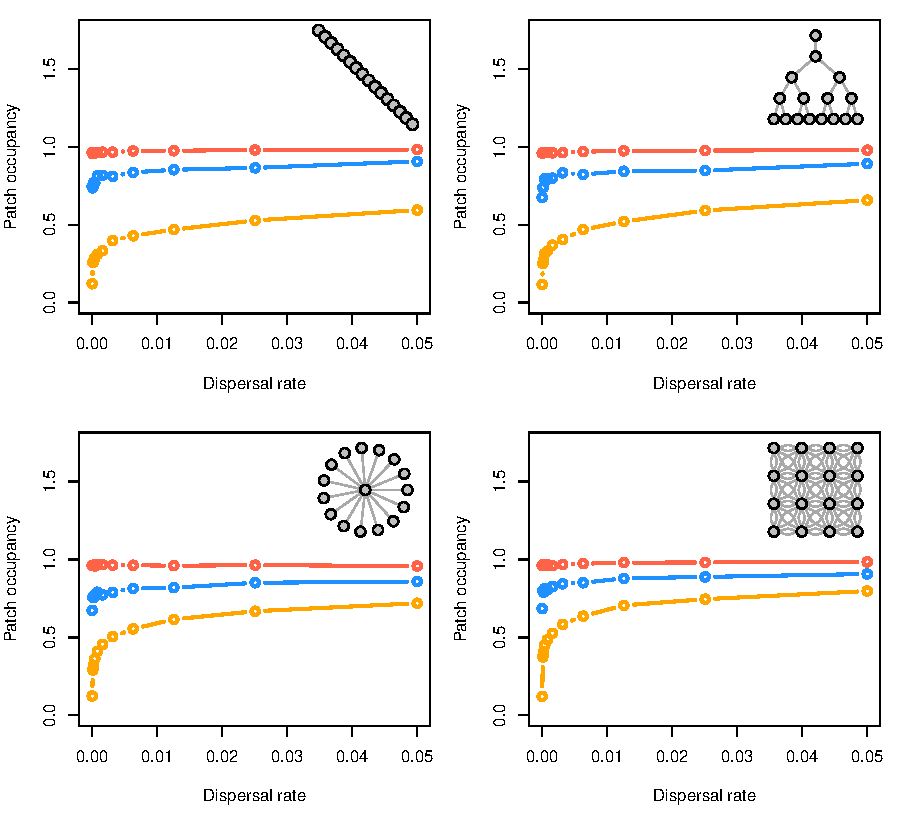
\includegraphics{Managing_for_ecological_surprises_in_metapopulations_files/figure-latex/patch occupancy with variable patches and stochasticity-1} 

}

\caption{Patch occupancy after 25 years along dispersal, disturbance (red - uniform; blue - localized, random; orange - localized, extirpation), and network gradients with variable patches and stochastic recruitment.}\label{fig:patch occupancy with variable patches and stochasticity}
\end{figure}

\newpage

\hypertarget{patch-occupancy-with-variable-patches-and-spatio-temporally-correlated-stochasticity-in-recruitment}{%
\paragraph{Patch occupancy with variable patches and spatio-temporally
correlated stochasticity in
recruitment}\label{patch-occupancy-with-variable-patches-and-spatio-temporally-correlated-stochasticity-in-recruitment}}

Now, we illustrate how variable patch demography and high
spatial-temporal correlations in stochastic recrtuitment affects
long-term patch occupancy.

\begin{figure}[H]

{\centering 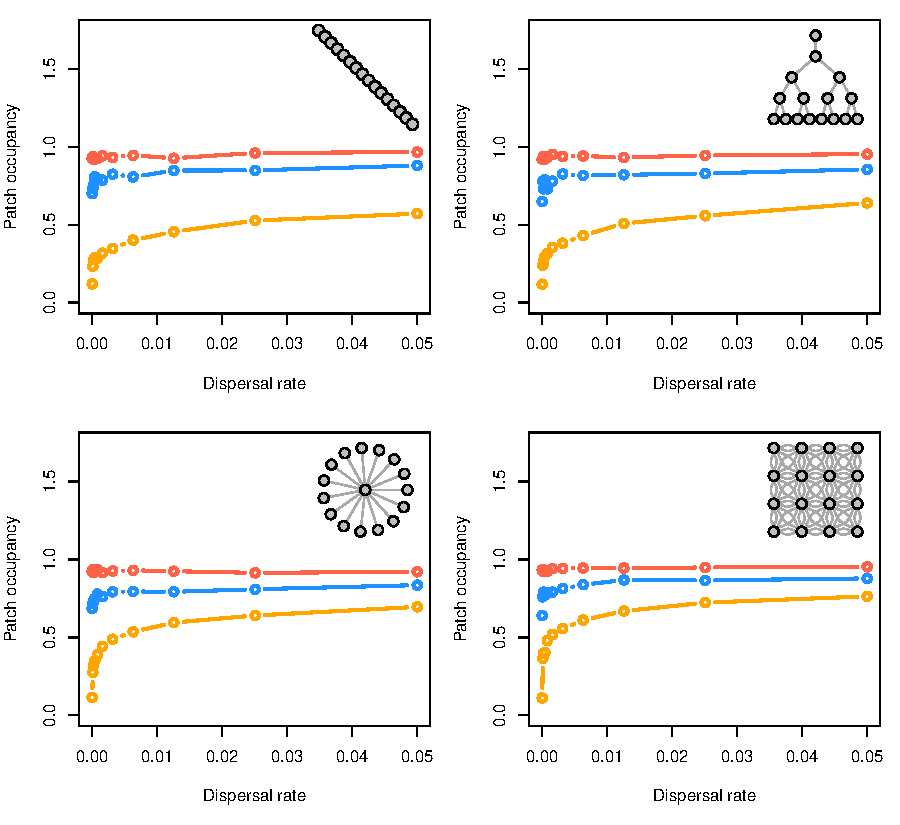
\includegraphics{Managing_for_ecological_surprises_in_metapopulations_files/figure-latex/patch occupancy with variable patches and space-time stochasticity-1} 

}

\caption{Patch occupancy after 25 years along dispersal, disturbance (red - uniform; blue - localized, random; orange - localized, extirpation), and network gradients with variable patches and spatial-temporal correlations in stochastic recruitment.}\label{fig:patch occupancy with variable patches and space-time stochasticity}
\end{figure}
\newpage

\hypertarget{references}{%
\subsection*{References}\label{references}}
\addcontentsline{toc}{subsection}{References}

\hypertarget{refs}{}
\leavevmode\hypertarget{ref-Anderson2015}{}%
Anderson, S.C., Moore, J.W., McClure, M.M., Dulvy, N.K. \& Cooper, A.B.
(2015). Portfolio conservation of metapopulations under climate change.
Ecological Applications 25 (2), 559-572. \emph{Ecological Applications},
\textbf{25}, 559--572.

\leavevmode\hypertarget{ref-igraph2006}{}%
Csardi, G. \& Nepusz, T. (2006). The igraph software package for complex
network research. \emph{InterJournal}, \textbf{Complex Systems}, 1695.

\leavevmode\hypertarget{ref-Forrest2010}{}%
Forrest, R.E., McAllister, M.K., Dorn, M.W., Martell, S.J. \& Stanley,
R.D. (2010). Hierarchical Bayesian estimation of recruitment parameters
and reference points for Pacific rockfishes (Sebastes spp.) under
alternative assumptions about the stock--recruit function.
\emph{Canadian Journal of Fisheries and Aquatic Sciences}, \textbf{67},
1611--1634.

\leavevmode\hypertarget{ref-Hanski1998}{}%
Hanski, I. (1998). Metapopulation dynamics. \emph{Nature}, \textbf{396},
41--49.

\leavevmode\hypertarget{ref-Yeakel2014}{}%
Yeakel, J.D., Moore, J.W., Guimarães, P.R. \& Aguiar, M.A. de. (2014).
Synchronisation and stability in river metapopulation networks.
\emph{Ecology Letters}, \textbf{17}, 273--283.


\end{document}
